\subsection{\texorpdfstring{空间 \(E_{A}\)（A 有界）}{空间 E\_\{A\}（A 有界）}}

设 E 是一个局部凸空间，A 是 E 的一个凸均衡子集。我们回忆，\(E_{A}\) 表示由 A 生成的向量空间，并以 A 的度规 \(p_{A}\) 作为半范数（II, 第 26 页, 例 3）。我们立即验证，\(E_{A}\) 到 E 中的典范单射连续，当且仅当 A 有界。此外，若 E 是 Hausdorff 的，则有界集 A 不包含任何直线（III, 第 2 页, 注 4），于是 \(p_{A}\) 是一个范数（II, loc. cit.）。

我们称一致空间 X 是半完备的，如果 X 中每个 Cauchy 序列都收敛。完备的一致空间是半完备的；但其逆并不总成立（GT, II, § 4, 习题 4）；不过，可度量化的半完备空间是完备的（GT, IX, § 2, No.~6, 命题 9）。

命题 8. --- 设 E 是一个 Hausdorff 局部凸空间，A 是 E 的一个闭的、均衡的、有界的且凸的子集。设 \((x_{n})\) 是 \(E_{A}\) 中的一个 Cauchy 序列。则此序列在 \(E_{A}\) 中收敛，当且仅当它在 E 中收敛。

\(E_{A}\) 到 E 中的典范单射是连续的。因此，若 \((x_{n})\) 在 \(E_{A}\) 中收敛，则它在 E 中收敛。反之，设 \((x_{n})\) 在 E 中收敛于 y。存在一个递增的整数序列 \((n_{k})\)，使得 \(p_{\mathbf{A}}(x_{m}-x_{n}) \leqslant 2^{-k-1}\) 成立，只要 \(m \geqslant n_{k}\) 且 \(n \geqslant n_{k}\)。于是序列 \((x_{n_{k}} + 2^{-k}\mathbf{A})\) 是递减的。由于 A 在 E 中是闭的，我们有 \(y \in \bigcap_{k} (x_{n_{k}} + 2^{-k}\mathbf{A})\)，这就证明了 \((x_{n_{k}})\)，从而 \((x_{n})\)，在 \(E_{A}\) 中收敛于 y。

推论. --- 若 A 是半完备的（特别是，完备的），则 \(E_{A}\) 是一个 Banach 空间。

事实上，\(E_{A}\) 中的一个 Cauchy 序列对 E 的拓扑而言也是 Cauchy 序列，并且含于一个与 A 位似的集合中，因此在 E 中收敛。

\subsection{完备有界集与拟完备空间}

定义 6. --- 称局部凸空间 E 是拟完备的，如果 E 的每个闭且有界的子集都是完备的（对由 E 的一致结构诱导的一致结构而言）。

完备的局部凸空间是拟完备的，但其逆并不总成立。* 例如，若 E 是一个无穷维 Hilbert 空间，或更一般地，是一个无穷维自反 Banach 空间，则赋弱化拓扑的 E 是拟完备的但不是完备的（II, 第 51 页, 命题 9）。*

拟完备空间是半完备的，因为每个 Cauchy 序列都含于一个闭且有界的子集中（III, 第 3 页, 推论与命题 1）。特别地，可度量化的拟完备局部凸空间是完备的。

在 Hausdorff 拟完备空间中，预紧子集的闭包与闭均衡凸包都是紧的；事实上，它们是预紧的（II, 第 25 页, 命题 3），并且因闭且有界而是完备的（III, 第 3 页, 命题 2）。

命题 9. --- (i) 拟完备局部凸空间的一个闭向量子空间是拟完备的。

\begin{enumerate}
\def\labelenumi{(\roman{enumi})}
\setcounter{enumi}{1}
\item
  拟完备局部凸空间的乘积是拟完备的。
\item
  拟完备局部凸空间的拓扑直和是拟完备的。
\item
  作为闭拟完备子空间的一个序列的严格归纳极限的局部凸空间是拟完备的。
\end{enumerate}

断言 (i) 由注 2（III, 第 2 页）得出，(ii) 由 III, 第 4 页, 推论 2 得出，(iii) 由命题 5（III, 第 5 页）得出，(iv) 由命题 6（III, 第 5 页）得出。

我们以后将看到，拟完备局部凸空间关于一个闭向量空间的商空间未必是拟完备的（IV, 第 63 页, 习题 10）。

命题 10. --- 设 E 是一个局部凸空间，M 是 E 的一个向量子空间，使得 E 的每个点都位于 M 的某个有界子集的闭包中。则从 M 到一个 Hausdorff 拟完备局部凸空间 F 中的每个连续线性映射 f 都唯一扩张为从 E 到 F 中的一个连续线性映射。

该假设蕴含 M 在 E 中稠密，于是 f 唯一扩张为从 E 到 F 的完备化 \(\hat{F}\) 中的一个连续线性映射 f（GT, III, § 3, No.~4, 推论）。但每个 \(x \in F\) 都位于 M 的某个有界子集 B 的闭包中；因此 \(\hat{f}(x)\) 位于 \(f(\mathbf{B})\) 在 \(\hat{F}\) 中的闭包内。而 \(f(\mathbf{B})\) 在 F 中有界，故它在 F 中的闭包是完备的，并且与它在 \(\hat{F}\) 中的闭包相一致。这就证明了 \(\hat{f}(x) \in \mathbf{F}\)。

\subsection{例}

\begin{enumerate}
\def\labelenumi{\alph{enumi})}
\tightlist
\item
  设 X 是一个拓扑空间。给 \(\mathcal{R}(\mathrm{X})\)，即 X 上（有限）数值函数所成的向量空间，赋予紧收敛拓扑（GT, X, §1, No.~3）：这是使诸限制映射 \(\mathcal{R}(\mathrm{X}) \to \mathcal{R}(\mathrm{H})\) 连续的最粗拓扑（其中 H 取遍 X 的紧子集族，而 \(\mathcal{R}(\mathrm{H})\) 赋予一致收敛拓扑）。III, 第 4 页 的推论 3 表明，\(\mathcal{R}(\mathrm{X})\) 的子集 A 有界，当且仅当对 X 的每个紧子集 H，属于 A 的函数在 H 上的限制所成之集是一致有界的。
\end{enumerate}

* b)（无穷可微函数空间。）设 \(n \geqslant 1\) 是一个整数。对 \(\mathbf{R}^n\) 中的每个开集 U，用 \(\mathcal{C}^\infty(\mathrm{U})\) 表示 U 上无穷可微函数所成的向量空间（VAR, R, 2.3）。设 \(f\) 属于 \(\mathcal{C}^\infty(\mathrm{U})\)。对每个多重指标 \(\alpha = (\alpha_1, \dots, \alpha_n)\)（属于 \(\mathbf{N}^n\)），用 \(\partial^\alpha f\) 表示偏导数 \(\partial^{|\alpha|} f / \partial x_1^{\alpha_1} \dots \partial x_n^{\alpha_1}\)；它是 U 上的一个连续函数（VAR, R, 2.3 与 2.4）。对每个整数 \(m \geqslant 0\) 以及 U 的每个紧子集 H，令

\[
p_{m,\mathrm{H}}(f) = \sup_{\substack{|\alpha |\leqslant m\\ x\in \mathrm{H}}}\left|\partial^{\alpha}f(x)\right|.\tag{1}
\]

于是 \(p_{m,\mathrm{H}}\) 是 \(\mathcal{C}^{\infty}(\mathrm{U})\) 上的一个半范数。

给 \(\mathcal{C}^{\infty}(\mathrm{U})\) 赋予由诸半范数 \(p_{m,\mathrm{H}}\) 所定义的拓扑。这是使诸映射 \(f\to \partial^{\alpha}f\)（从 \(\mathcal{C}^{\infty}(\mathrm{U})\) 到 \(\mathcal{R}(\mathrm{U})\) 中，其中 \(\mathcal{R}(\mathrm{U})\) 赋予紧收敛拓扑）连续的最粗拓扑。存在 U 的紧子集的一个递增序列 \((\mathrm{H}_n)_{n\geqslant 0}\)，它们的内部覆盖 U；半范数族 \(p_{m,\mathrm{H}_n}\) 定义了 \(\mathcal{C}^{\infty}(\mathrm{U})\) 的拓扑，后者于是成为一个可度量化的局部凸空间。空间 \(\mathcal{C}^{\infty}(\mathrm{U})\) 是完备的；换言之，它是一个 Fréchet 空间（II, 第 24 页）：事实上，设 \((f_k)\) 是 \(\mathcal{C}^{\infty}(\mathrm{U})\) 中的一个 Cauchy 序列；对每个 \(\alpha \in \mathbf{N}^n\)，序列 \((\partial^{\alpha}f_k)\) 在完备空间 \(\mathcal{R}(\mathrm{U})\) 中收敛（TG, X, §1, No.~5, 定理 1）于一个连续函数 \(g_{\alpha}\)。对 \(|\alpha|\) 作归纳，我们由 FVR, II, 第 2 页 的定理 1 推出 \(g_{\alpha} = \partial^{\alpha}g_{0}\) 对每个 \(\alpha \in \mathbf{N}^n\) 成立。换言之，序列 \((f_k)\) 收敛于 \(g_0\)（在 \(\mathcal{C}^{\infty}(\mathrm{U})\) 中）。

设 A 是 \(\mathcal{C}^{\infty}(\mathrm{U})\) 的一个子集。要使 A 有界，其充分必要条件是：数 \(\sup_{f\in \mathbf{A}}p_{m,\mathrm{H}}(f)\) 对每个整数 \(m\geqslant 0\) 以及每个

  U 的紧子集 H 而言都是有限的；这一条件意味着：对每个 \(\alpha\in \mathbf{N}^{n}\)，诸函数 \(\partial^{\alpha}f|H\)（\(f\in A\)）所成之集对每个紧的 \(H\subset U\) 都是一致有界的。

设 \(\mathrm{H} \subset \mathrm{U}\) 是紧的。用 \(\mathcal{C}_{\mathrm{H}}^{\infty}(\mathrm{U})\) 表示 \(\mathcal{C}^{\infty}(\mathrm{U})\) 中由支集含于 \(\mathrm{H}\) 的那些函数所组成的子空间。空间 \(\mathcal{C}_{\circ}^{\infty}(\mathrm{U})\)，即 \(\mathrm{U}\) 中具有紧支集的无穷可微函数所成的空间，是诸子空间 \(\mathcal{C}_{\mathrm{H}}^{\infty}(\mathrm{U})\) 的递增有向并，其中 \(\mathrm{H}\) 取遍 \(\mathrm{U}\) 的紧子集族。每个空间 \(\mathcal{C}_{\mathrm{H}}^{\infty}(\mathrm{U})\) 都赋予由 \(\mathcal{C}^{\infty}(\mathrm{U})\) 的拓扑诱导的拓扑，而 \(\mathcal{C}_{\circ}^{\infty}(\mathrm{U})\) 赋予相应的归纳极限拓扑。如果诸集 \(\mathrm{H}_n\) 的内部构成 \(\mathrm{U}\) 的一个覆盖，那么空间 \(\mathcal{C}_{\circ}^{\infty}(\mathrm{U})\) 是诸 Fréchet 空间 \(\mathcal{C}_{\mathrm{H}_n}^\infty (\mathrm{U})\) 的严格归纳极限；因此它是完备的（II, 第 32 页, 命题 9），并且 \(\mathcal{C}_{\circ}^{\infty}(\mathrm{U})\) 的每个有界子集都含于诸子空间 \(\mathcal{C}_{\mathrm{H}_n}^\infty (\mathrm{U})\) 之一（III, 第 5 页, 命题 6）。*

\begin{enumerate}
\def\labelenumi{\alph{enumi})}
\setcounter{enumi}{2}
\tightlist
\item
  （Gevrey 空间。）设 I 是 \(\mathbf{R}\) 中的一个紧区间。对每个整数 \(n \geqslant 0\)，用 \(\mathrm{D}^n f\) 表示定义在 I 上的数值函数的 \(n\) 阶导数（该函数为 \(f\)，只要此导数存在）。设 \(s \geqslant 1\) 与 \(\mathbf{M} \geqslant 0\) 是两个实数。用 \(\mathcal{G}_{s,\mathbf{M}}(\mathrm{I})\) 表示 I 上满足如下条件的那些无穷可微函数 \(f\)（FVR, I, 第 28 页）所成的向量空间：序列 \((|\mathrm{D}^n f| / \mathrm{M}^n (n!)^s)_{n \geqslant 0}\) 在 I 上所有连续函数所成的空间 \(\mathcal{C}(\mathrm{I})\)（赋一致收敛拓扑）中是有界的。空间 \(\mathcal{G}_{s,\mathbf{M}}(\mathrm{I})\) 赋予下述范数后是一个 Banach 空间
\end{enumerate}

\[
\| f \| _ {s, \mathbf {M}} = \sup _ {n \geqslant 0, x \in \mathrm{I}} | \mathrm{D} ^ {n} f (x) | / \mathrm{M} ^ {n} (n!) ^ {s}.
\]

对 \(\mathbf{M} \leqslant \mathbf{M}'\)，我们有 \(\mathcal{G}_{s,\mathbf{M}}(\mathrm{I}) \subset \mathcal{G}_{s,\mathbf{M}'}(\mathrm{I})\)，并且

\[
\| f \| _ {s, \mathbf {M} ^ {\prime}} \leqslant \| f \| _ {s, \mathbf {M}}
\]

对每个 \(f \in \mathcal{G}_{s,\mathsf{M}}(\mathrm{I})\) 成立。用 \(\mathcal{G}_s(\mathrm{I})\) 表示诸空间 \(\mathcal{G}_{s,\mathsf{M}}(\mathrm{I})\) 的并，并给它赋予 \(\mathcal{G}_{s,\mathsf{M}}(\mathrm{I})\) 的诸拓扑的归纳极限拓扑。

设 \(M < M'\)，并设 B 是 \(\mathcal{G}_{s,M}(I)\) 中的（闭）单位球。我们将证明 B 是 Banach 空间 \(\mathcal{G}_{s,M'}(I)\) 的一个紧子集。显然 B 在 \(\mathcal{G}_{s,M'}(I)\) 中是闭的，故只需证明 B 在 \(\mathcal{G}_{s,M'}(I)\) 中是预紧的。设 \(\varepsilon > 0\)，并设 N 是使 \((M/M')^N \leqslant \varepsilon/2\) 的一个正整数。设 k 是一个正整数；当 f 取遍 B 时，诸函数 \(D^{k+1}f\) 所成之集在 \(\mathcal{C}(I)\) 中是有界的，因而当 f 取遍 B 时，诸函数 \(D^k f\) 所成之集在 \(\mathcal{C}(I)\) 中是相对紧的：这由有限增量定理（FVR, I, 第 23 页, 推论 1）以及 Ascoli 定理（GT, X, § 2, No.~5）得出。我们在 \(\mathcal{G}_{s,M}(I)\) 上借助下式定义一个范数

\[
q(f) = \sup_{\substack{0\leqslant n\leqslant \mathbf{N}\\ x\in \mathrm{I}}}\big|\mathrm{D}^{n}f(x)\big| / \mathrm{M}^{\prime n}(n!)^{s}  .
\]

上述论证表明，B 对于范数 q 相应的拓扑而言是预紧的；换言之，存在 B 的一个有限子集 C，使得对每个 \(f \in B\)，存在 \(g \in C\) 满足 \(q(f - g) \leqslant \varepsilon\)。最后，对每个 n \textgreater{} N，我们有

\[
\left| \mathrm{D} ^ {n} f (x) - \mathrm{D} ^ {n} g (x) \right| / \mathrm{M} ^ {\prime n} (n!) ^ {s} \leqslant 2 (\mathrm{M} / \mathrm{M} ^ {\prime}) ^ {n} \leqslant \varepsilon ,
\]

由此得到 \(\| f - g\| \leqslant \varepsilon\)。这就证明了 B 在 \(\mathcal{G}_{s,M'}(I)\) 中是预紧的。

空间 \(\mathcal{G}_s(\mathrm{I})\) 是诸空间 \(\mathcal{G}_{s,k}(\mathrm{I})\)（当 \(k\) 取遍 \(\mathbf{N}\) 时）的归纳极限；由命题 7（III, 第 6 页），\(\mathcal{G}_s(\mathrm{I})\) 的每个有界子集都含于诸空间 \(\mathcal{G}_{s,k}(\mathrm{I})\) 之一，并且在这个空间中是相对紧的。

* \(d\) )（全纯函数空间。）设 \(n \geqslant 1\) 是一个整数。对 \(\mathbf{C}^n\) 的每个开子集 U，\(\mathcal{H}(\mathrm{U})\) 表示在 U 中全纯的函数所成的空间，并赋予 U 中紧收敛拓扑。对 \(\mathbf{C}^n\) 的每个紧子集 L，\(\mathcal{H}(\mathrm{L})\) 表示在 L 的一个邻域中全纯的函数的芽所成的空间；我们给这个空间赋予使诸典范映射 \(\pi_{\mathrm{U}}:\mathcal{H}(\mathrm{U})\to\mathcal{H}(\mathrm{L})\) 连续的最细局部凸拓扑，其中 U 取遍 L 的开邻域所成之集。

对每个整数 \(m \geqslant 1\)，设 \(U_{m}\) 是 \(C^{n}\) 中与 L 的距离 \textless{} 1/m 的点所成之集。可以证明，典范映射 \(\pi_{U_{m}}\)（从 \(\mathcal{H}(U_{m})\) 到 \(\mathcal{H}(L)\) 中）是单射，并且从 \(\mathcal{H}(U_{m})\) 到 \(\mathcal{H}(U_{p})\) 中的限制映射对 \(p \geqslant m\) 是紧的。于是可以应用命题 7（III, 第 6 页）。设 A 是 \(\mathcal{H}(L)\) 的一个有界子集；则存在一个整数 \(m \geqslant 1\)，使得 A 由 L 的一个邻域中函数的芽组成，这些函数属于 \(\mathcal{H}(U_{m})\) 中的一个有界集 B。此外，映射 \(\phi\)（从 \(\mathcal{H}(L)\) 到一个拓扑空间 T 中）连续，当且仅当映射 \(\phi \circ \pi_{U}\)（从 \(\mathcal{H}(U)\) 到 T 中）对 L 的每个开邻域 U 都连续。*

\section{有界型空间}

在本节中，E 表示一个局部凸空间，B 表示它的典范有界结构（III, 第 3 页, 定义 5）。

引理 1. --- 设 G 是一个半赋范空间，p 是它的半范数，u 是从 G 到 E 中的一个线性映射。下列条件等价：

\begin{enumerate}
\def\labelenumi{(\roman{enumi})}
\item
  \(u\) 连续；
\item
  \(G\) 的单位球在 \(u\) 下的像在 \(\mathbf{E}\) 中是有界的；
\item
  对每个趋于 0 的点序列 \((x_{n})\)（诸点属于 \(\mathbf{G}\)），序列 \((u(x_{n}))\) 在 E 中有界。
\end{enumerate}

立即可见 (i) 蕴含 (ii)（III, 第 4 页, 推论 1），并且 (ii) 蕴含 (iii)。设 V 是 E 中 0 的一个邻域；如果 \(u^{-1}(\mathrm{V})\) 不是 G 中 0 的邻域，那么存在点的一个序列 \((y_n)\)，其诸点属于 \(\mathrm{G} - u^{-1}(\mathrm{V})\)，使得 \(p(y_n) \leqslant \frac{1}{n^2}\)。于是序列 \(x_n = ny_n\) 在 G 中趋于 0，且 \(u(x_n) \notin n\mathrm{V}\)，这蕴含序列 \((u(x_n))\) 不是有界的。因此 (iii) 蕴含 (i)。

命题 1. -- 下列条件等价：

\begin{enumerate}
\def\labelenumi{(\roman{enumi})}
\tightlist
\item
  \(\mathbf{E}\) 上每个在 \(\mathbf{E}\) 的有界子集上有界的半范数都是连续的。
\end{enumerate}

(i') E 的吸收 E 的诸有界子集（I, 第 7 页, 定义 4）的每个凸均衡子集都是 E 中 0 的一个邻域。

\begin{enumerate}
\def\labelenumi{(\roman{enumi})}
\setcounter{enumi}{1}
\tightlist
\item
  E 是诸半赋范空间 \(E_{A}\) 的归纳极限，其中 A 取遍 E 的闭的、凸的、均衡的且有界的子集所成的递增有向集。
\end{enumerate}

(ii') 存在半赋范空间的一个族 \((\mathrm{E}_{i})_{i\in\mathrm{I}}\)，并且对每个 \(i\in I\)，存在一个线性映射 \(u_{i}:E_{i}\to E\)，使得 E 的拓扑是使诸 \(u_{i}\) 连续的最细局部凸拓扑。

\begin{enumerate}
\def\labelenumi{(\roman{enumi})}
\setcounter{enumi}{2}
\tightlist
\item
  对任意的局部凸空间 F，线性映射 \(u: E \to F\) 连续，当且仅当对 E 中趋于 0 的每个点序列 \((x_{n})\)，序列 \((u(x_{n}))\) 在 F 中有界。
\end{enumerate}

(iii') 对任意的半赋范空间 \(\mathbf{F}\)，线性映射 \(u: \mathbf{E} \to \mathbf{F}\) 连续，当且仅当 \(u(\mathbf{X})\) 在 \(\mathbf{F}\) 中有界，其中 \(\mathbf{X}\) 取遍 \(\mathbf{E}\) 中的有界集。

鉴于半范数与凸的、均衡的、吸收的子集之间的对应（II, 第 20 页），立即可见 (i) 与 (i') 等价。若 \(p\) 是 E 上的一个半范数，它在每个 \(\mathrm{E}_{\mathrm{A}}\) 上连续，则 \(p\) 在 E 的有界子集上有界；因而 (i) 蕴含 (ii)（II, 第 27 页, 命题 5）。显然 (ii) 蕴含 (ii')。

现在设 \((\mathrm{E}_{i}, u_{i})_{i\in I}\) 如 (ii') 所述，并设 u 是从 E 到一个局部凸空间 F 中的一个线性映射，使得 \((u(x_{n}))\) 在 F 中有界，对 E 中趋于 0 的每个点序列 \((x_{n})\) 皆然。由 III, 第 11 页 的引理 1 推出，线性映射 \(u\circ u_{i}:E_{i}\to F\) 对所有 \(i\in I\) 连续。因此，若 E 的拓扑是使诸 \(u_{i}\) 连续的最细局部凸拓扑，则 u 连续（II, 第 27 页, 命题 5）。这就证明了 (ii') 蕴含 (iii)。

立即可见 (iii) 蕴含 (iii')（III, 第 3 页, 推论）。最后，若 \(p\) 是 E 上的一个半范数，它在 E 的有界子集上有界，则条件 (iii') 断言恒等映射从 E 到半赋范空间 (E, \(p\)) 中连续；换言之，\(p\) 连续。这就证明了 (iii') 蕴含 (i)。

定义 1. --- 称局部凸空间为有界型空间，如果它满足命题 1 的诸等价条件。

例. --- 1) 每个半赋范空间都是有界型空间。

\begin{enumerate}
\def\labelenumi{\arabic{enumi})}
\setcounter{enumi}{1}
\item
  特别地，每个有限维局部凸空间都是有界型空间。
\item
  由于终局部凸拓扑的传递性（II, 第 28 页, 推论 2），我们由条件 (ii') 立即推出：若 \((\mathrm{E}_i)_{i\in I}\) 是有界型局部凸空间的一个族，且给 E 赋予使诸线性映射 \(u_{i}:\mathrm{E}_{i}\to \mathrm{E}\)（对 \(i\in \mathrm{I}\)）连续的最细局部凸拓扑，则 E 是有界型空间。特别地，有界型空间的归纳极限、直和、商空间都是有界型空间。
\end{enumerate}

另一方面，有界型空间的闭子空间未必是有界型空间（IV, 第 63 页, 习题 8）。

推论. --- 每个 Hausdorff 且半完备的有界型空间都是 Banach 空间的一个归纳极限。

事实上，其中 A 闭且有界的那些空间 \(E_{A}\) 都是 Banach 空间（III, 第 8 页, 推论）。

命题 2. --- 局部凸可度量化空间是有界型空间。

设 E 可度量化，p 是 E 上的一个半范数，它在 E 的有界子集上有界，但不连续。设 A 是所有 \(x \in E\) 中使 \(p(x) < 1\) 者构成的集。设 \((\mathrm{V}_{n})_{n \geqslant 1}\) 是构成 E 中 0 的一个基本邻域系的递减序列。由于 p 不连续，A 不是 0 的邻域；因而对每个 n \textgreater{} 0，有 \(A \not\subset n^{-1}V_{n}\)，且存在一点 \(x_{n}\) 位于 \(V_{n}\) 中，使得 \(n^{-1}x_{n} \notin A\)，即 \(p(x_{n}) \geqslant n\)。序列 \((x_{n})\) 趋于 0，故有界（III, 第 3 页, 推论）；这与关于 p 的假设矛盾。

推论. --- 每个 Fréchet 空间（II, 第 24 页）都是 Banach 空间的一个归纳极限。

\section{连续线性映射空间}

\subsection{\texorpdfstring{空间 \(\mathcal{L}_{\mathfrak{S}}(\mathbf{E};\mathbf{F})\)}{空间 \textbackslash mathcal\{L\}\_\{\textbackslash mathfrak\{S\}\}(\textbackslash mathbf\{E\};\textbackslash mathbf\{F\})}}

设 \(\mathbf{F}\) 是一个拓扑向量空间，\(\mathbf{E}\) 是一个任意集合，\(\mathfrak{S}\) 是 \(\mathbf{E}\) 的子集的一个族。考虑向量空间 \(\mathrm{F}^{\mathrm{E}}\)，带上 \(\mathfrak{S}\) -收敛的一致结构（GT, X, § 1, No.~2）。我们知道这一结构与 \(\mathrm{F}^{\mathrm{E}}\) 的交换群结构相容（GT, X, § 1, No.~4, 推论 2）。如此得到的拓扑称为 \(\mathfrak{S}\) -拓扑。若 \(\mathbf{X}\) 是 \(\mathrm{F}^{\mathrm{E}}\) 的一个子集，或更一般地，是带有映射 \(j: \mathrm{X} \to \mathrm{F}^{\mathrm{E}}\) 的一个集合，则在 \(j\) 之下，\(\mathfrak{S}\) -拓扑（于 \(\mathrm{F}^{\mathrm{E}}\) 上）的原像称为 \(\mathfrak{S}\) -拓扑（在 \(\mathbf{X}\) 上）。

注. --- 1) \(\mathfrak{S}\) -拓扑与 \(\mathfrak{S}'\) -拓扑相同，其中 \(\mathfrak{S}'\) 表示由 \(\mathfrak{S}\) 生成的有界结构（III, 第 1 页）。

\begin{enumerate}
\def\labelenumi{\arabic{enumi})}
\setcounter{enumi}{1}
\tightlist
\item
  设 \(\mathbf{M} \in \mathfrak{S}\)，并设 \(\mathbf{V}\) 是 \(\mathbf{F}\) 中 0 的一个邻域；用 \(\mathrm{T}(\mathbf{M}, \mathbf{V})\) 表示所有这样的 \(f \in \mathrm{F}^{\mathrm{E}}\) 所成的集：\(f(x) \in \mathbf{V}\) 对每个 \(x \in \mathbf{M}\) 成立。若 \(\mathfrak{S}\) 在有限并下稳定，则诸集 \(\mathrm{T}(\mathbf{M}, \mathbf{V})\) 构成 \(\mathfrak{S}\) -拓扑（\(\mathrm{F}^{\mathrm{E}}\) 的）的 0 的一个基本邻域系。
\end{enumerate}

命题 1. --- 设 E 是一个集合，S 是 E 的子集的一个族，F 是一个拓扑向量空间，H 是 \(F^{E}\) 的一个向量子空间。为使 S-拓扑与 H 的向量空间结构相容，必要且充分的是 \(u(\mathbf{M})\) 对每个 \(u \in H\) 和每个 \(M \in S\) 都在 F 中有界。此外，若 F 是局部凸的，则 H 上的 S-拓扑是局部凸的。

根据上面的注 1) 和 2)，我们看到 \(\mathfrak{S}\) -拓扑与 H 的向量空间结构相容的一个必要且充分条件是：诸集 \(\mathrm{H} \cap \mathrm{T}(\mathbf{M}, \mathrm{V})\) 在 H 中是吸收的（I, 第 7 页, 命题 4）；但这蕴含着：对每个 \(u \in \mathrm{H}\)、每个子集 \(\mathbf{M} \in \mathfrak{S}\) 以及 F 中 0 的每个均衡邻域 V，存在 \(\lambda \neq 0\) 使得 \(u(M) \subset \lambda V\)；也就是说（III, 第 2 页），\(u(\mathbf{M})\) 在 F 中有界。最后，命题的最后一个断言由如下事实得出：若 V 是凸的，则 \(\mathrm{T}(\mathbf{M}, \mathrm{V})\) 也是凸的。

推论. --- 设 E 与 F 是两个局部凸空间，S 是 E 的有界子集的一个族，\(\mathcal{L}(E; F)\) 是从 E 到 F 中的连续线性映射所成的向量空间。则 S-拓扑与 \(\mathcal{L}(E; F)\) 的向量空间结构相容且是局部凸的。

只需指出：若 \(u\) 是从 \(\mathbf{E}\) 到 \(\mathbf{F}\) 中的一个连续线性映射，且 \(\mathbf{M}\) 是 \(\mathbf{E}\) 的一个有界子集，则 \(u(\mathbf{M})\) 在 \(\mathbf{F}\) 中有界（III, 第 4 页, 推论 1）。

给定两个局部凸向量空间 E 和 F 以及 E 的有界子集的一个族 S，用 \(\mathcal{L}_{\mathfrak{S}}(E;F)\) 表示给 \(\mathcal{L}(E;F)\) 赋予 S-拓扑所得到的局部凸空间。

例. --- 1) 若 \(\mathfrak{S}\) 是 E 的所有有限子集所成的集，则 \(\mathfrak{S}\) -拓扑是简单收敛拓扑，且空间 \(\mathcal{L}_{\mathfrak{S}}(E; F)\) 也记作 \(\mathcal{L}_s(E; F)\)。\(\mathcal{L}_s(E; F)\) 的一个有界子集称为 \(\mathcal{L}(E; F)\) 的一个简单有界子集。

\begin{enumerate}
\def\labelenumi{\arabic{enumi})}
\setcounter{enumi}{1}
\item
  若 \(\mathfrak{S}\) 是紧（相应地，预紧、紧凸）子集所成的集，则 \(\mathfrak{S}\) -拓扑称为紧（相应地，预紧、紧凸）收敛拓扑，且空间 \(\mathcal{L}_{\mathfrak{S}}(\mathrm{E};\mathrm{F})\) 也记作 \(\mathcal{L}_c(\mathrm{E};\mathrm{F})\)（相应地，\(\mathcal{L}_{pc}(\mathrm{E};\mathrm{F}),\mathcal{L}_{cc}(\mathrm{E};\mathrm{F})\)）。（参见 IV, 第 48 页, 习题 7。）
\item
  若 \(\mathfrak{S}\) 是 E 的所有有界子集所成的集，我们说 \(\mathfrak{S}\) -拓扑是有界收敛拓扑，且空间 \(\mathcal{L}_{\mathfrak{S}}(\mathrm{E};\mathrm{F})\) 记作 \(\mathcal{L}_b(\mathrm{E};\mathrm{F})\)。
\item
  当 \(\mathrm{F} = \mathbf{K}\) 时，空间 \(\mathcal{L}(\mathrm{E};\mathrm{F})\) 就是 \(\mathrm{E}'\)，也就是 \(\mathrm{E}\) 的对偶。我们用 \(\mathrm{E}_{\Xi}^{\prime}, \mathrm{E}_{s}^{\prime}\) 等表示空间 \(\mathcal{L}_{\Xi}(\mathrm{E};\mathbf{K}), \mathcal{L}_s(\mathrm{E};\mathbf{K})\) 等。空间 \(\mathrm{E}_s^\prime\)（相应地，\(\mathrm{E}_b^\prime\)）称为 \(\mathrm{E}\) 的弱对偶（相应地，强对偶）。\(\mathrm{E}_s^\prime\)（相应地，\(\mathrm{E}_b^\prime\)）的一个有界子集称为弱有界（相应地，强有界）的。我们注意到 \(\mathrm{E}'\) 上的弱拓扑不是别的，正是 \(\sigma (\mathrm{E}',\mathrm{E})\)（II, 第 42 页）。
\end{enumerate}

当 \(\mathrm{E} = \mathrm{F}\) 时，我们用 \(\mathcal{L}(\mathrm{E}), \mathcal{L}_{\mathfrak{S}}(\mathrm{E})\) 等表示空间 \(\mathcal{L}(\mathrm{E};\mathrm{F}), \mathcal{L}_{\mathfrak{S}}(\mathrm{E};\mathrm{F})\) 等。设 \(p\) 是 \(\mathrm{F}\) 上的一个连续半范数，\(\mathbf{M}\) 是 \(\mathrm{E}\) 的一个有界子集。设

\[
p _ {\mathrm{M}} (u) = \sup _ {x \in \mathrm{M}} p (u (x)).\tag{1}
\]

立即可见 \(p_{M}\) 是 \(\mathcal{L}(E;F)\) 上的一个半范数，并且若 \(\Gamma\) 是 F 上的一个基本半范数系，则半范数族 \(p_{M}\)（其中 p 取遍 \(\Gamma\)，M 取遍由 S 生成的有界结构的一个基）是 \(\mathcal{L}_{\mathfrak{S}}(E;F)\) 的一个基本半范数系。

特别地，若 E 和 F 是半赋范空间，且 p（相应地，q）表示 E（相应地，F）的半范数，则 \(\mathcal{L}(\mathrm{E};\mathrm{F})\) 上的有界收敛拓扑由半范数

\[
r (u) = \sup _ {p (x) \leqslant 1} q (u (x))\tag{2}
\]

（参见 GT, X, § 3, No.~2）。当我们把 \(\mathcal{L}_b(\mathrm{E};\mathrm{F})\) 看作半赋范空间时，除非另有明确说明，我们总是指半范数 (2)。若 F 是赋范空间，则半范数 (2) 是一个范数。

注. --- 3) 设 A 是 E 的单位球的一个稠密子集。鉴于 u 的连续性，我们还有

\[
r (u) = \sup _ {x \in \mathrm{A}} q (u (x)).\tag{3}
\]

例如

\[
r (u) = \sup _ {p (x) <   1} q (u (x)).\tag{4}
\]

由于 \(u(tx) = tu(x)\) 对 \(t \in \mathbf{R}\) 成立，我们还有，

\[
r (u) = \sup _ {p (x) = 1} q (u (x)) = \sup _ {p (x) \neq 0} \frac {q (u (x))}{p (x)}.\tag{5}
\]

只要 \(p \neq 0\)。

\begin{enumerate}
\def\labelenumi{\arabic{enumi})}
\setcounter{enumi}{3}
\tightlist
\item
  公式 (2) 表明映射 \(u \mapsto r(u)\) 在 \(\mathcal{L}_s(\mathrm{E};\mathrm{F})\) 上是下半连续的。
\end{enumerate}

命题 2. --- 设 E 和 F 是两个局部凸空间，并设 S 是 E 的有界子集所成的一个集。

\begin{enumerate}
\def\labelenumi{\arabic{enumi})}
\item
  \(\mathfrak{S}\) -拓扑（\(\mathcal{L}(\mathrm{E};\mathrm{F})\) 上的）与 \(\mathfrak{S}\) -拓扑相同，其中 \(\mathfrak{S}\) 表示 \(\mathrm{E}\) 上包含 \(\mathfrak{S}\) 的最小适配有界结构（III, 第 3 页）。
\item
  假设 \(\{0\}\) 在 \(\mathbf{F}\) 中不稠密，并设 \(\mathfrak{S}'\) 是 \(\mathbf{E}\) 的有界子集所成的另一个集。则 \(\mathfrak{S}'\) -拓扑粗于 \(\mathfrak{S}\) -拓扑，当且仅当 \(\mathfrak{S}' \subset \tilde{\mathfrak{S}}\)。
\end{enumerate}

设 \(u \in \mathcal{L}(\mathrm{E};\mathrm{F})\)，\(\mathbf{M} \in \mathfrak{S}\)，并设 \(p\) 是 \(\mathrm{F}\) 上的一个连续半范数。由于 \(p \circ u\) 是 \(\mathrm{E}\) 上的连续半范数，这就等于说 \(p \circ u\) 在 \(\mathbf{M}\) 上、或在闭凸均衡包 \(\tilde{\mathbf{M}}\)（\(\mathbf{M}\) 的）上以 1 为上界；换言之，我们有 \(p_{\mathbf{M}} = p_{\tilde{\mathbf{M}}}\)。此外，显然我们有 \(p_{\lambda \mathbf{M}} = \lambda p_{\mathbf{M}}\)（对所有 \(\lambda > 0\)），且有 \(p_{\mathbf{M} \cup \mathbf{M}'} = \sup(p_{\mathbf{M}}, p_{\mathbf{M}'})\)，由此即得第一个断言，因为 \(\tilde{\mathfrak{S}}\) 以 \(\mathfrak{S}\) 中集合的有限并的闭凸均衡包的位似所成之集为一个基。

我们现在证明第二个断言：首先，若 \(\mathbf{F}\) 是基域，则由定义可得，\(\tilde{\mathfrak{S}}\) -拓扑（在 \(\mathrm{E}' = \mathcal{L}(\mathrm{E};\mathrm{F})\) 上）以 \(\tilde{\mathfrak{S}}\) 中诸集的极集所成之集为 0 的一个基本邻域系。设 \(\mathbf{A}\) 是 \(\mathbf{E}\) 的一个有界子集，其极集 \(\mathbf{A}^{\circ}\) 是 \(\tilde{\mathfrak{S}}\) -拓扑下 0 的一个邻域；则存在闭凸均衡集 \(\mathbf{B} \in \tilde{\mathfrak{S}}\) 使得 \(\mathbf{A}^{\circ} \supset \mathbf{B}^{\circ}\)，于是 \(\mathbf{A} \subset \mathbf{B}^{\circ \circ}\)；但由 II, 第 45 页 的推论 3，有 \(\mathbf{B}^{\circ \circ} = \mathbf{B}\)，因此 \(\mathbf{A} \subset \mathbf{B}\) 且 \(\mathbf{A} \in \tilde{\mathfrak{S}}\)。于是，若 \(\mathfrak{S}'\) 是 \(\mathbf{E}\) 的有界子集所成的一个集，则 \(\mathfrak{S}'\) -拓扑粗于 \(\mathfrak{S}\) -拓扑（\(\mathrm{E}'\) 上的），当且仅当 \(\mathfrak{S}' \subset \tilde{\mathfrak{S}}\)。一般情形立即可得，因为若 \(y \in F\) 不在 0 的闭包中，则可以验证：使 \(f \in E'\) 对应于映射 \(x \mapsto f(x)y\) 的映射是局部凸空间 \(\mathrm{E}'_{\mathfrak{S}}\) 到它在 \(\mathcal{L}_{\mathfrak{S}}(\mathrm{E};\mathrm{F})\) 中的像上的一个同构。

\subsection{\texorpdfstring{\(\mathcal{L}_{\mathfrak{S}}(\mathbf{E};\mathbf{F})\) 为 Hausdorff 的条件}{\textbackslash mathcal\{L\}\_\{\textbackslash mathfrak\{S\}\}(\textbackslash mathbf\{E\};\textbackslash mathbf\{F\}) 为 Hausdorff 的条件}}

命题 3. -- 设 E 和 F 是两个局部凸空间，其中 F 假设为 Hausdorff 的，并设 \(\mathfrak{S}\) 是 E 的有界子集的一个族。若 \(\mathfrak{S}\) 中诸集的并 A 在 E 中是完全的，则空间 \(\mathcal{L}_{\mathfrak{S}}(\mathrm{E};\mathrm{F})\) 是 Hausdorff 的。

设 \(u_0\) 是 \(\mathcal{L}(\mathrm{E};\mathrm{F})\) 中一个非零元素；由于 \(u_0\) 连续且 \(\mathrm{A}\) 在 \(\mathrm{E}\) 中是完全的，存在一点 \(x_0\) 在 \(\mathrm{A}\) 中，使得 \(u_0(x_0) \neq 0\)。由于 \(\mathrm{F}\) 是 Hausdorff 的，存在 0 的一个邻域 \(\mathrm{V}\)（在 \(\mathrm{F}\) 中）使得 \(u_0(x_0) \notin \mathrm{V}\)。设 \(\mathbf{M} \in \mathfrak{S}\) 满足 \(x_0 \in \mathbf{M}\)。于是集 \(\mathrm{U}\)（由所有 \(u \in \mathcal{L}(\mathrm{E};\mathrm{F})\) 中使 \(u(\mathbf{M}) \subset \mathbf{V}\) 者组成）是 \(\mathcal{L}(\mathrm{E};\mathrm{F})\) 中 0 的一个邻域，且我们有 \(u_0 \notin \mathrm{U}\)，从而 \(\mathcal{L}(\mathrm{E};\mathrm{F})\) 是 Hausdorff 的。

特别地，只要 F 是 Hausdorff 的，\(\mathcal{L}(\mathrm{E};\mathrm{F})\) 上的下列拓扑就都是 Hausdorff 的：简单收敛、紧收敛、预紧或紧凸收敛，以及有界收敛拓扑。

\subsection{\texorpdfstring{\(\mathcal{L}(\mathbf{E};\mathbf{F})\) 与 \(\mathcal{L}(\hat{\mathbf{E}};\mathbf{F})\) 之间的关系}{\textbackslash mathcal\{L\}(\textbackslash mathbf\{E\};\textbackslash mathbf\{F\}) 与 \textbackslash mathcal\{L\}(\textbackslash hat\{\textbackslash mathbf\{E\}\};\textbackslash mathbf\{F\}) 之间的关系}}

设 E 和 F 是两个 Hausdorff 局部凸空间，并假设 F 完备；设 \(\hat{E}\) 是 E 的完备化。由于从 E 到 F 中的每个连续线性映射 u 都唯一地扩张为一个连续线性映射 \(\overline{u}\)（从 \(\hat{E}\) 到 F 中），我们可以把空间 \(\mathcal{L}(E;F)\) 与 \(\mathcal{L}(\hat{E};F)\) 通过映射 \(u\mapsto\overline{u}\) 等同起来。此外，设 S 是 E 的有界子集的一个族；\(\mathcal{L}(E;F)\) 上的 S-拓扑与 \(\mathcal{L}(\hat{E};F)\) 上的 S-拓扑重合，也与 \(\hat{S}\) -拓扑重合，其中 \(\hat{S}\) 表示 S 中诸集在 \(\hat{E}\) 中的闭包所成的族。

例如，若 E 是赋范的，则 \(\mathcal{L}(\mathrm{E};\mathrm{F})\) 上的有界收敛拓扑与 \(\mathcal{L}(\hat{\mathrm{E}};\mathrm{F})\) 上的有界收敛拓扑相同：因为 \(\hat{E}\) 的每个有界子集都包含在 E 的某个有界子集的闭包中。由于 \(\hat{E}\) 的单位球是 E 的单位球的闭包，由公式 (3)（III, 第 14 页）可得：若 F 是 Banach 空间，则映射 \(u\mapsto\overline{u}\) 是从 \(\mathcal{L}(\mathrm{E};\mathrm{F})\) 到 \(\mathcal{L}(\hat{\mathrm{E}};\mathrm{F})\) 上的一个等距。

我们注意到，若 E 不是赋范空间，则可能存在 \(\hat{E}\) 的有界子集，它不含于 E 的任何有界子集的闭包之中（例如，当 E 是无限维 Banach 空间的弱对偶时）；然而，若 E 可度量化且满足第一可数公理，则此事成立（III, 第 39 页, 习题 16）。

\subsection{\texorpdfstring{\(\mathcal{L}(\mathbf{E};\mathbf{F})\) 的等度连续子集}{\textbackslash mathcal\{L\}(\textbackslash mathbf\{E\};\textbackslash mathbf\{F\}) 的等度连续子集}}

设 \(\mathrm{E}\) 和 \(\mathrm{F}\) 是两个局部凸空间。为使子集 \(\mathrm{H}\)（\(\mathcal{L}(\mathrm{E};\mathrm{F})\) 的）等度连续，必要且充分的是它在 \(\mathrm{E}\) 中的点 0 处等度连续（I, 第 9 页, 命题 6）；这蕴含：对 0 的每个邻域 \(\mathrm{V}\)（在 \(\mathrm{F}\) 中），集 \(\bigcap_{u\in \mathrm{H}}u^{-1}(\mathrm{V})\) 是 \(\mathrm{E}\) 中 0 的一个邻域；或者，对每个连续半范数

\(p\)（\(\mathrm{F}\) 上的），函数 \(\sup_{u\in \mathrm{H}}(p\circ u)\) 是 E 上的连续半范数。此外（I, 第 5 页），

  H 是一致等度连续的。我们注意到，等度连续子集的凸均衡包是等度连续的，因为若 p 是 F 上的连续半范数而 \(\tilde{H}\) 是 H 的凸均衡包，则对 H 中的 \(u_{i}\)，有不等式 \(p \circ (\sum_{i} \lambda_{i} u_{i}) \leqslant \sum_{i} |\lambda_{i}| \cdot (p \circ u_{i})\)，因而 \(\sup_{u \in \tilde{H}} (p \circ u) = \sup_{u \in H} (p \circ u)\)。

因此，等度连续子集的族是 \(\mathcal{L}(\mathrm{E};\mathrm{F})\) 上的一个凸有界结构（III, 第 2 页, 定义 2）。

命题 4. --- 设 E、F 是两个局部凸空间，且 F 是 Hausdorff 的。给从 E 到 F 中的所有映射所成的空间 \(F^{E}\) 赋予简单收敛拓扑。则

\begin{enumerate}
\def\labelenumi{(\roman{enumi})}
\item
  从 \(\mathbf{E}\) 到 \(\mathbf{F}\) 中的线性映射所成之集在 \(\mathbf{F}^{\mathrm{E}}\) 中是闭的。
\item
  若 \(\mathbf{H}\) 是 \(\mathcal{L}(\mathrm{E};\mathrm{F})\) 的一个等度连续子集，则闭包 \(\overline{\mathbf{H}}\)（\(\mathbf{H}\) 在 \(\mathrm{F}^{\mathrm{E}}\) 中的）含于 \(\mathcal{L}(\mathrm{E};\mathrm{F})\) 且是等度连续的。
\end{enumerate}

我们知道 \(\overline{\mathbf{H}}\) 是等度连续的（GT, X, § 2, No.~3, 命题 6）。剩下要证明断言 (i)。设 \(x, y\) 在 E 中且 \(\lambda, \mu\) 在 K 中，并设 \(\mathbf{A}(x, y, \lambda, \mu)\) 是所有满足下式的 \(u \in \mathbf{F}^{\mathrm{E}}\) 所成之集：

\[
u (\lambda x + \mu y) - \lambda u (x) - \mu u (y) = 0.
\]

这个集在 \(F^{E}\) 中是闭的，因为映射 \(u \mapsto u(x)\)（从 \(F^{E}\) 到 F 中）对每个 \(x \in E\) 连续，且 \(F\) 是 Hausdorff 的。但从 \(E\) 到 \(F\) 中的线性映射所成之集等于

\[
\bigcap_ {x, y, \lambda , \mu} \mathrm{A} (x, y, \lambda , \mu).
\]

于是这个集在 \(F^{E}\) 中是闭的。

推论 1. --- 为使 \(\mathcal{L}(\mathrm{E};\mathrm{F})\) 的等度连续子集 H 在 \(\mathcal{L}_s(\mathrm{E};\mathrm{F})\) 中相对紧，必要且充分的是：对所有 \(x\in \mathrm{E}\)，集 \(\mathrm{H}(x)\)（由所有 \(u(x)\)（当 \(u\) 取遍 \(\mathrm{H}\)）组成）在 \(\mathrm{F}\) 中相对紧。

事实上，这个条件对 \(\overline{\mathbf{H}}\) 在 \(\mathrm{F}^{\mathrm{E}}\) 中紧是必要且充分的（GT, I, § 9, No.~5, 推论）。

推论 2. --- 对偶 E' 的每个等度连续子集在 E' 上的弱拓扑 \(\sigma(E', E)\) 下相对紧（III, 第 14 页, 例 4）。

因为若 H 是 \(E'\) 的一个等度连续子集，则 \(\sup_{u\in H}|u|\) 是 E 上的连续半范数；特别地，对每个 \(x\in E\)，集 \(\mathrm{H}(x)\) 有界，从而在标量域中相对紧。

推论 3. --- 在半赋范空间 E 的强对偶 \(E_{b}^{\prime}\) 中，每个闭球对弱拓扑 \(\sigma(\mathrm{E}^{\prime},\mathrm{E})\) 都是紧的。

这个球对 \(\sigma(\mathrm{E}^{\prime},\mathrm{E})\) 也是闭的。

命题 5. --- 设 E 和 F 是两个局部凸空间，并设 T 是 E 的一个完全子集。下列一致结构在 \(\mathcal{L}(\mathrm{E};\mathrm{F})\) 的每个等度连续子集 H 上重合：

\begin{enumerate}
\def\labelenumi{\arabic{enumi})}
\item
  T 上的简单收敛一致结构；
\item
  E 上的简单收敛一致结构；
\item
  在 E 的预紧子集上收敛的一致结构。
\end{enumerate}

我们回忆（III, 第 15 页, 命题 2）：\(\mathfrak{S}\) -拓扑（\(\mathcal{L}(\mathrm{E};\mathrm{F})\) 上的）与 \(\tilde{\mathfrak{S}}\) -拓扑重合，其中 \(\tilde{\mathfrak{S}}\) 是适配于 E 且包含 \(\mathfrak{S}\) 的最小有界结构。

因此在命题 5 的陈述中，我们可以把「完全」一词换成「处处稠密」。于是该命题由等度连续集的一般性质得出（GT, X, § 2, No.~4, 定理 1）。

例. --- * 1) 设 \(\mu\) 是 \(\mathbf{R}\) 上的 Lebesgue 测度，并设 E 是半赋范空间 \(\mathcal{L}^p(\mu)\)（\(1 \leqslant p < \infty\)）（INT, IV）。对每个数值函数 \(f\) 和每个实数 \(h\)，设 \(f_h\) 为函数 \(x \mapsto f(x - h)\)。显然映射 \(f \mapsto f_h\) 定义了 E 到它自身上的一个线性等距。若 \(f\) 连续且有紧支集，则 \(f_h\) 一致收敛于 \(f\)，从而也以 \(p\) 阶平均收敛（当 \(h\) 趋于 0 时）。由于所有具有紧支集的连续函数所成之集 \(\mathcal{K}(\mathbf{R})\) 在 E 中稠密，且 E 的线性等距所成之集是等度连续的，由命题 5 可得：对每个 \(f \in E\)，\(f_h\) 以 \(p\) 阶平均收敛于 \(f\)（当 \(h\) 趋于 0 时）。

对 \(p = 1\)，考虑 Fourier 变换，它使每个 \(f \in \mathcal{L}^1(\mu)\) 对应于函数 \(\hat{f}\)（定义在 \(\mathbf{R}\) 上），后者由下式定义

\[
\hat {f} (y) = \int e ^ {- 2 i \pi x y} f (x) d \mu (x).
\]

线性型 \(f \mapsto \hat{f}(y)\) 所成之集是 \(\mathcal{L}^1(\mu)\) 的对偶的一个等度连续子集。另一方面，我们知道闭有界区间的特征函数所成之集 \(T\) 是 \(\mathcal{L}^1(\mu)\) 的一个完全子集；并且容易验证：对所有 \(f \in T\)，Fourier 变换 \(\hat{f}\) 是一个连续函数且在无穷远处趋于零。我们推出这对所有 \(f \in \mathcal{L}^1(\mu)\) 都成立（「Riemann-Lebesgue 定理」）。

关系式 \(\sup_{y\in \mathbb{R}}|\hat{f} (y)|\leqslant \| f\| _1\) 表明映射 \(f\mapsto \hat{f}\) 是一个连续映射

它从 \(\mathcal{L}^1 (\mu)\) 映入空间 \(\mathcal{B}(\mathbf{R})\)（即 \(\mathbf{R}\) 上所有有界函数所成的空间），后者带有一致收敛结构。由于 \(\hat{f}\) 对所有 \(f\in \mathrm{T}\) 连续，由此得出 \(\hat{f}\) 对所有 \(f\in \mathcal{L}^1 (\mu)\) 连续。\(\hat{f}\) 在无穷远处趋于零这一事实由如下事实得出：在无穷远处趋于零的所有连续函数所成的子空间 \(\mathcal{C}_0(\mathbf{R})\) 在 \(\mathcal{B}(\mathbf{R})\) 中是闭的。

\begin{enumerate}
\def\labelenumi{\arabic{enumi})}
\setcounter{enumi}{1}
\tightlist
\item
  设 E 是 R 上所有连续数值函数所成的空间，带上紧收敛拓扑。设 K 是 R 的一个紧子集，并设 \((\mu_{n})\) 是 R 上支集含于 K 的测度的一个序列。假设对所有 n 有 \(\|\mu_{n}\|\leqslant1\)。于是诸 \(\mu_{n}\) 所成之集是 \(E'\) 的一个等度连续子集。因此，若对每个函数 \(f\in E\) 有 \(\lim_{n\to\infty}\mu_{n}(f)=0\)，则函数序列 \(x\mapsto\int e^{itx}d\mu_{n}(t)\) 收敛于 0，
\end{enumerate}

且在 \(\mathbf{R}\) 的每个紧子集上一致收敛（因为诸函数 \(t \mapsto e^{itx}\)——当 \(x\) 取遍 \(\mathbf{R}\) 的一个紧子集时——所成之集在 E 中是紧的）。*

推论. --- 假设 F 是 Hausdorff 的。设 H 是 \(\mathcal{L}(\mathrm{E};\mathrm{F})\) 的一个等度连续子集。若 H 上的一个滤子 \(\Phi\) 简单收敛到一个从 E 到 F 中的映射 \(u_{0}\)，则 \(u_{0}\) 是从 E 到 F 中的一个连续线性映射，且 \(\Phi\) 在 E 的每个预紧子集上一致收敛于 \(u_{0}\)。

第一个断言由命题 4（III, 第 16 页）得出，第二个由命题 5（III, 第 17 页）得出。

命题 6. --- 设 H 是 \(\mathcal{L}(\mathrm{E};\mathrm{F})\) 的一个等度连续子集。若 F 可度量化且 E 中存在一个可数完全集，则 H 上 E 中简单收敛的一致结构是可度量化的。若此外 F 中还存在一个可数完全集，则 H 中存在一个可数的处处稠密集（对 E 的紧子集上的一致收敛拓扑而言）。

设 \((a_{n})\) 是 E 中的一个完全序列。则映射 \(u \mapsto (u(a_{n}))\) 是从 \(\mathcal{L}(\mathrm{E};\mathrm{F})\)（其中 \(\mathcal{L}(\mathrm{E};\mathrm{F})\) 带有诸 \(a_{n}\) 所成之集上简单收敛的一致结构）到 \(F^{N}\) 的一个一致子空间上的一个同构。若 F 可度量化（相应地，可度量化且满足第一可数公理），则 \(F^{N}\) 亦然（GT, IX, § 2, No.~4, 推论 2 及 § 2, No.~8, 推论），而命题由命题 5（III, 第 17 页）得出。

推论 1. --- 设 E 是一个局部凸可度量化空间，F 是一个赋范空间。假设 E 和 F 都满足第一可数公理。则 \(\mathcal{L}(\mathrm{E};\mathrm{F})\) 是可数个等度连续子集所成的族的并，且在 \(\mathcal{L}(\mathrm{E};\mathrm{F})\) 中存在一个可数集，它对 E 的预紧子集上的一致收敛拓扑是稠密的。

设 B 是 F 的单位球，\((\mathrm{V}_{n})\) 是 E 中 0 的一个可数基本邻域系。对每个整数 n，集 \(H_{n}\)（由所有 \(u \in \mathcal{L}(\mathrm{E}; \mathrm{F})\) 中使 \(u(\mathrm{V}_{n}) \subset \mathrm{B}\) 者组成）是等度连续的，且 \(\mathcal{L}(\mathrm{E}; \mathrm{F})\) 是诸 \(H_{n}\) 的并。于是该推论由命题 6 得出。

推论 2. --- 在满足第一可数公理的赋范空间的对偶 E' 中，每个闭球对弱拓扑 \(\sigma(\mathrm{E}',\mathrm{E})\) 都是一个紧可度量化空间，且对该拓扑，E' 中存在一个可数稠密子集。

这由命题 6 以及 III, 第 17 页, 推论 3 得出。

\subsection{\texorpdfstring{\(\mathbf{E}'\) 的等度连续子集}{\textbackslash mathbf\{E\}\textquotesingle{} 的等度连续子集}}

在本节中，E 表示一个局部凸空间，\(E'\) 表示其对偶。每当我们谈到一个集 M 的极 \(M^{\circ}\)（M 位于 E 中，相应地，位于 \(E'\) 中）时，除非另有说明，我们总是指相对于 E 与 \(E'\) 之间的对偶而言的 M 的极。回忆：若 V 是 E 中 0 的一个闭凸均衡邻域，我们有 \(V^{\circ\circ}=V\)（II, 第 45 页, 推论 3）。

命题 7. --- 设 M 是 E' 的一个子集。下列条件等价：

\begin{enumerate}
\def\labelenumi{(\roman{enumi})}
\item
  M 是等度连续的；
\item
  \(\mathbf{M}\) 含于 E 中 0 的一个邻域的极中；
\item
  \(\mathbf{M}\) 的极是 E 中 0 的一个邻域。
\end{enumerate}

若 \(\mathbf{M}\) 等度连续，则存在 0 的一个凸均衡邻域 \(V\)，使得 \(|u(x)| \leqslant 1\) 对所有 \(x \in V\) 及所有 \(u \in M\) 成立；于是我们有 \(\mathbf{M} \subset V^{\circ}\)，从而 (i) 蕴含 (ii)。用同样的记号，若 \(\mathbf{M} \subset V^{\circ}\)，则 \(\mathbf{V} \subset V^{\circ \circ} \subset M^{\circ}\)，从而 (ii) 蕴含 (iii)。最后，若 \(\mathbf{M}^{\circ}\) 包含 0 的一个凸均衡邻域 \(V\)，则 \(\mathbf{M} \subset M^{\circ \circ} \subset V^{\circ}\)，且关系 \(x \in \varepsilon V\)、\(u \in M\) 蕴含 \(|u(x)| \leqslant \varepsilon\)（对所有 \(\varepsilon > 0\)），这就证明了 (iii) 蕴含 (i)。

我们注意到，每个 \(x \in E\) 定义了一个映射 \(j(x): u \mapsto u(x)\)，它从 \(E'\) 到 K 中。因此我们可以谈论 E 上的 S-拓扑，其中 S 是 \(E'\) 的子集的一个族：这是 \(K^{E'}\) 上的 S-拓扑在 j 下的原像。我们立即验证：若 S 是 \(E'\) 上的一个凸有界结构，则 S 中诸集的极构成 E 上 S-拓扑的 0 的一个基本邻域系。特别地，当 S 是 \(E'\) 的等度连续子集的族时即是如此，且命题 7 蕴含：

推论 1. --- E 的拓扑与在 E' 的等度连续子集上一致收敛的拓扑相同。

更一般地，设 F 是一个局部凸空间；每个 \(u \in \mathcal{L}(\mathrm{E}; \mathrm{F})\) 定义了一个映射 \(j(u):(x, f) \mapsto f(u(x))\)，它从 \(E \times F'\) 到 K 中（即到 R 或 C 中）。这使我们能够在空间 \(\mathcal{L}(\mathrm{E}; \mathrm{F})\) 上定义在 \(E \times F'\) 的子集所成之集上一致收敛的拓扑。特别地：

推论 2. --- 设 S 是 E 的有界子集的一个族。\(\mathcal{L}(\mathrm{E};\mathrm{F})\) 上的 S-拓扑是在形如 \(\mathbf{A}\times\mathbf{B}\subset\mathbf{E}\times\mathbf{F}'\) 的集合上一致收敛的拓扑，其中 A 属于 S，而 B 属于 F' 的等度连续子集的族。

对每个 \(u \in \mathcal{L}(\mathrm{E}; \mathrm{F})\)、每个 \(A \in S\) 以及 F 中 0 的每个闭凸均衡邻域 V，关系 \(u(\mathrm{A}) \subset \mathrm{V}\) 等价于 \(\ll j(u) (\mathrm{A} \times \mathrm{V}^{\circ})\) 含于 K 的单位球中 \(\gg\)。

命题 8. --- 设 H 是从 E 到一个局部凸空间 F 中的线性映射的一个族。为使 H 等度连续，必要且充分的是：对 F 的对偶 F' 中每个等度连续子集 X，线性型 \(f \circ u\)（\(f \in X\) 且 \(u \in H\)）所成之集是等度连续的。

显然该条件是必要的。假设它成立，并设 V 是 F 中 0 的一个闭凸均衡邻域。由于 \(V^{\circ}\) 等度连续，存在 E 中 0 的一个邻域 W，使得 \(\left|f(u(x))\right| \leqslant 1\) 对所有 \(x \in W\)、\(u \in H\) 及 \(f \in V^{\circ}\) 成立；换言之，\(u(W) \subset V^{\circ\circ} = V\) 对所有 \(u \in H\) 成立，故 H 等度连续。

\subsection{局部凸空间的完备化}

定理 1（Grothendieck）. --- 设 E 是一个局部凸空间，并设 S 是 E 上一个适配且覆盖的有界结构。设 \(F \subset E^{*}\) 是 E 上这样的线性型所成的空间：它们在每个属于 S 的集上的限制是连续的。若给 F 赋予 S-拓扑，则从 \(E'_{S}\) 到 F 中的典范单射扩张为从完备化 \(\hat{E}'_{S}\)（即 \(E'_{S}\) 的完备化）到 F 上的一个同构。

由于 E 上线性型的每个简单极限是线性型（III, 第 16 页, 命题 4），且 E 上的有界结构 \(\mathfrak{S}\) 是覆盖的，由 GT, X, § 1, No.~6, 推论 2 可得：带 \(\mathfrak{S}\) -拓扑的空间 F 是 Hausdorff 且完备的。显然 \(E_{\mathfrak{S}}'\) 是 F 的一个拓扑向量子空间；因此只需证明 \(E_{\mathfrak{S}}'\) 在 F 中处处稠密。这由下面的引理得出：

引理 1. --- 设 A 是 E 的一个闭凸均衡子集，并设 u 是 E 上的一个线性型，它在 A 上的限制连续。则对每个 \(\varepsilon > 0\)，存在一个 \(x' \in E'\) 使得

\[
\left| u (x) - \langle x, x ^ {\prime} \rangle \right| \leqslant \varepsilon \quad \text { for   every } \quad x \in A.
\]

设 \(\varepsilon > 0\)。存在 E 中 0 的一个闭凸均衡邻域 U，使得 \(|u(x)| \leqslant \varepsilon\) 对所有 \(x \in \mathrm{U} \cap \mathrm{A}\) 成立。我们知道极 \(\mathrm{U}^{\circ}\)（U 在 \(\mathrm{E}^{*}\) 中的）含于 \(\mathrm{E}'\) 且对拓扑 \(\sigma(\mathrm{E}^{*}, \mathrm{E})\) 是紧的（III, 第 17 页, 推论 2）。由于极 \(\mathrm{A}^{\circ}\)（A 在 \(\mathrm{E}^{*}\) 中的）对 \(\sigma(\mathrm{E}^{*}, \mathrm{E})\) 是闭的，由此得出 \(\mathrm{A}^{\circ} + \mathrm{U}^{\circ}\) 是 \(\mathrm{E}^{*}\) 的一个闭凸子集（GT, III, § 4, No.~1, 推论 1）。

设 C 是 E 的一个闭凸均衡子集。则 C 对 \(\sigma(\mathrm{E},\mathrm{E}^{\prime})\) 是闭的（II, 第 45 页, 推论 3），从而对 \(\sigma(\mathrm{E},\mathrm{E}^{*})\) 也是闭的，因而我们有 \(C = C^{\circ\circ}\)（对 E 与 \(E^{*}\) 之间的对偶而言）。结果，我们有

\[
\mathrm{A} \cap \mathrm{U} = \mathrm{A} ^ {\circ \circ} \cap \mathrm{U} ^ {\circ \circ} = (\mathrm{A} ^ {\circ} \cup \mathrm{U} ^ {\circ}) ^ {\circ} \supset (\mathrm{A} ^ {\circ} + \mathrm{U} ^ {\circ}) ^ {\circ}
\]

由此得到

\[
(\mathrm{A} \cap \mathrm{U}) ^ {\circ} \subset (\mathrm{A} ^ {\circ} + \mathrm{U} ^ {\circ}) ^ {\circ \circ} = \mathrm{A} ^ {\circ} + \mathrm{U} ^ {\circ}.
\]

由于线性型 \(\varepsilon^{-1}u\) 属于 \((\mathrm{A}\cap\mathrm{U})^{\circ}\)，存在 \(v\in A^{\circ}\) 及 \(w\in U^{\circ}\) 使得 \(u=\varepsilon(v+w)\)。于是 \(x'=\varepsilon w\) 属于 \(E'\)，且 \(u-x'=\varepsilon v\) 在 A 上的绝对值以 \(\varepsilon\) 为上界；引理得证。

现在设 E 是一个局部凸 Hausdorff 空间，\(\hat{E}\) 是它的完备化。E 上每个连续线性型 f 由连续性扩张到 \(\hat{E}\)：因而我们有 \((\hat{\mathrm{E}})' = \mathrm{E}'\)（III, 第 16 页），且 \(\hat{\mathbf{E}}\) 的每个元素定义了 \(\mathbf{E}'\) 上的一个线性型；也就是说，定义了代数对偶 \(\mathbf{E}^{\prime *}\)（\(\mathbf{E}'\) 的）的一个元素。此外，\(\mathbf{E}\)（相应地，\(\hat{\mathbf{E}}\)）与 \(\mathbf{E}'\) 之间的对偶是分离的（II, 第 24 页, 推论 1）。因此 \(\mathbf{E}\) 与 \(\hat{\mathbf{E}}\) 可与 \(\mathbf{E}^{\prime *}\) 的向量子空间等同起来。

定理 2. --- 设 E 是一个局部凸 Hausdorff 空间，\(\hat{\mathbf{E}}\) 是它的完备化；我们把 E 与 \(\hat{\mathbf{E}}\) 与 \(\mathbf{E}^{\prime *}\) 的向量子空间等同起来。则为使元素 \(f \in \mathbf{E}^{\prime *}\) 属于 \(\hat{\mathbf{E}}\)，必要且充分的是：\(f\) 在 \(\mathbf{E}'\) 的每个等度连续子集上的限制对拓扑 \(\sigma(\mathbf{E}', \mathbf{E})\) 连续。

空间 E 可与 \(E'\) 的拓扑对偶等同起来，当给 \(E'\) 赋予拓扑 \(\sigma(E', E)\) 时（II, 第 43 页, 命题 3）；另一方面，若 S 是 \(E'\) 的等度连续子集所成之集，则 E 上给定的拓扑就是 S-拓扑（III, 第 19 页, 推论 1）。于是由 III, 第 13 页, 命题 1 可得，S 的诸集对 \(\sigma(E', E)\) 有界（参见后面 III, 第 22 页, 命题 9）；换言之，S 是对拓扑 \(\sigma(E', E)\) 而言适配且覆盖的有界结构。若把 E 换成 \(E'\) 并把 \(E'_{S}\) 换成 E，则定理 2 是定理 1 的推论。

推论 1（Banach）. --- 设 E 是一个 Hausdorff 且完备的局部凸空间。为使 \(E'\) 上的一个线性型对弱拓扑 \(\sigma(E', E)\) 连续（即由 E 的一个元素产生），只需它在 \(E'\) 的每个等度连续子集上的限制对 \(\sigma(E', E)\) 连续。

评注. --- 此外假设 E 中存在一个可数完全集；则 \(E'\) 的每个等度连续子集对拓扑 \(\sigma(E', E)\) 可度量化（III, 第 18 页, 命题 6）；因此为验证 \(E'\) 上的线性型 u 是弱连续的，只需验证：对每个等度连续序列 \((x_{n}')\)（在 \(E'\) 中且对 \(\sigma(E', E)\) 收敛于 0），我们有 \(\lim_{n \to \infty} u(x_{n}') = 0\)。

推论 2. --- 设 \((\mathrm{E}_{i})_{i\in\mathbb{I}}\) 是 Hausdorff 局部凸空间的一个族，并设 E 是它们的拓扑直和。则从诸 \(\hat{E}_{i}\) 的直和到 \(\hat{E}\) 中的典范映射是一个同构。特别地，E 完备当且仅当所有 \(E_{i}\) 都完备。

我们知道 E 的对偶可与诸 \(E_{i}\) 的对偶的乘积等同起来（II, 第 30 页, 公式 (1)）。设 \(u \in \hat{E}\)，并设 \(u_{i} \in E_{i}^{\prime *}\) 是 u（视为 \(E^{\prime *}\) 的元素）在 \(E_{i}^{\prime} \subset E^{\prime}\) 上的限制。立即可见，只需证明：\(u_{i} = 0\) 除有限多个指标 \(i \in I\) 外成立。反之，假设存在一个由互异指标构成的序列 \((i_{n})_{n \in \mathbf{N}}\) 使得 \(u_{i_{n}} \neq 0\)。则存在 \(x_{i_{n}} \in E_{i_{n}}^{\prime}\) 使得 \(u_{i_{n}}(x_{i_{n}}) = n\)。所有 \(x_{i_{n}}\) 所成之集 H 在 \(E^{\prime}\) 中等度连续，而 u 在 H 上的限制不是有界的，这是不可能的。

\subsection{\texorpdfstring{\(\mathcal{L}(\mathbf{E};\mathbf{F})\) 上的 S-有界结构}{\textbackslash mathcal\{L\}(\textbackslash mathbf\{E\};\textbackslash mathbf\{F\}) 上的 S-有界结构}}

设 E 和 F 是两个局部凸空间，S 是 E 的有界子集的一个族。说 \(\mathcal{L}(E; F)\) 的子集 H 对 S-拓扑有界，意思是对每个 \(\mathbf{M} \in \mathfrak{S}\)，0 的每个邻域 \(V\)（在 \(F\) 中）吸收集 \(\mathrm{H(M)} = \bigcup_{u \in H} u(\mathrm{M})\)；这等于说，对每个 \(\mathbf{M} \in \mathfrak{S}\)，集 \(\mathrm{H(M)}\) 在 \(F\) 中有界。等价地，这意味着对 0 的每个邻域 \(V\)（在 \(F\) 中），集 \(\bigcap_{u \in H} u^{-1}(V)\)

吸收 S 的每个子集 M。

命题 9. --- 设 E 和 F 是两个局部凸空间，S 是 E 的有界子集的一个族。则 \(\mathcal{L}(\mathrm{E};\mathrm{F})\) 的每个等度连续子集对 S-拓扑有界。

因为若 \(\mathbf{H}\) 是 \(\mathcal{L}(\mathrm{E};\mathrm{F})\) 的一个等度连续子集，且 \(\mathbf{V}\) 是 \(\mathbf{F}\) 中 0 的一个邻域，则集 \(\bigcap_{u\in \mathbf{H}}u^{-1}(\mathbf{V})\) 是 \(\mathbf{E}\) 中 0 的一个邻域，故吸收 \(\mathbf{E}\) 的每个有界子集。

\(\mathcal{L}(\mathrm{E};\mathrm{F})\) 中对某个 S-拓扑有界的子集未必等度连续，即使 S 是覆盖的且 S 是 E 上的典范有界结构（IV, 第 50 页, 习题 17）。在下一段中我们将以桶型空间之名研究这样的空间 E：\(\mathcal{L}(\mathrm{E};\mathrm{F})\) 的每个简单有界子集都是等度连续的。目前请注意下面的结果：

命题 10. --- 设 E 是一个有界型空间（特别地，是可度量化的局部凸空间），F 是一个局部凸空间。\(\mathcal{L}(\mathrm{E};\mathrm{F})\) 中对有界收敛拓扑有界的每个子集 H 都是等度连续的。

对 F 中 0 的每个凸均衡邻域 V，集 \(\bigcap_{u\in\mathbf{H}}u^{-1}(\mathbf{V})\) 吸收 E 的每个有界子集，故是 E 中 0 的一个邻域；这就证明了 H 等度连续。

\subsection{\texorpdfstring{\(\mathcal{L}_{\mathfrak{S}}(\mathbf{E};\mathbf{F})\) 的完备子集}{\textbackslash mathcal\{L\}\_\{\textbackslash mathfrak\{S\}\}(\textbackslash mathbf\{E\};\textbackslash mathbf\{F\}) 的完备子集}}

命题 11. --- 设 E 和 F 是两个局部凸空间，S 是由有界子集组成的 E 的一个覆盖。若 F 是 Hausdorff 且拟完备的（III, 第 8 页），则 \(\mathcal{L}(\mathrm{E};\mathrm{F})\) 中对 S-拓扑为闭的每个等度连续子集 H 都是 \(\mathcal{L}_{\mathfrak{S}}(\mathrm{E};\mathrm{F})\) 的一个完备一致子空间。

由于 H 在 \(\mathcal{L}_{\mathfrak{S}}(\mathrm{E};\mathrm{F})\) 中有界（III, 第 22 页, 命题 9），且在 \(F^{E}\) 中对 S-拓扑为闭（III, 第 16 页, 命题 4），这由 GT, X, § 1, No.~5 的推论 3 得出。

注 1. --- 设 M 是 \(\mathcal{L}_{\mathfrak{S}}(\mathrm{E};\mathrm{F})\) 的一个完备一致子空间。对 E 的有界子集所成的每个集 \(\mathfrak{S}' \supset \mathfrak{S}\)，\(\mathfrak{S}'\) -拓扑细于 \(\mathfrak{S}\) -拓扑（在 \(\mathcal{L}(\mathrm{E};\mathrm{F})\) 上）；另一方面，存在 \(\mathfrak{S}'\) -拓扑的 0 的一个基本邻域系，其中的邻域对简单收敛拓扑是闭的（III, 第 13 页, 注 2），从而更对 \(\mathfrak{S}\) -拓扑是闭的。我们断定（GT, III, § 3, No.~5, 推论 1）M 对 \(\mathfrak{S}'\) -拓扑是完备的。

推论. --- 设 E 和 F 是两个局部凸空间，H 是 \(\mathcal{L}(\mathrm{E};\mathrm{F})\) 的一个等度连续子集。若 F 是 Hausdorff 且拟完备的，且 H 上的一个滤子 \(\Phi\) 在 E 的一个完全子集 T 的所有点处简单收敛，则存在从 E 到 F 中的一个连续线性映射 u，使得 \(\Phi\) 在 E 的每个预紧子集上一致收敛于 u。

因为由命题 5（III, 第 17 页），\(\Phi\) 是 E 上预紧收敛一致结构的一个 Cauchy 滤子；由命题 11，H 的闭包 \(\overline{\mathrm{H}}\)（在 \(\mathcal{L}_{pc}(\mathrm{E};\mathrm{F})\) 中）是完备的，从而 \(\Phi\) 在 E 的每个预紧子集上一致收敛到一个映射 \(u\in \overline{\mathrm{H}}\)。

注 2. --- 设 \((u_{n})\) 是从一个 Banach 空间 E 到一个 Banach 空间 F 中的连续线性映射的一个序列；可能发生这样的情况：\((u_{n}(x))\) 在 E 的一个处处稠密的向量子空间 T 的每点处都有极限，而序列 \((u_{n})\) 在赋范空间 \(\mathcal{L}(\mathrm{E};\mathrm{F})\) 中并不有界。例如，取 E 为 R 上所有在无穷远处趋于零的连续数值函数所成的空间，带上范数 \(\|f\| = \sup_{x \in \mathbf{R}} |f(x)|\)，并设 T 为连续数值函数的子空间

它由具有紧支集者组成。从 E 到 R 中的连续线性映射 \(f \mapsto nf(n)\) 的序列对所有 \(f \in T\) 收敛于 0，但在 \(\mathcal{L}_{b}(E; \mathbf{R})\) 中不有界。同一个例子表明：在空间 \(\mathcal{L}(T; \mathbf{R})\) 中，一个序列 \((v_{n})\) 可以是简单收敛的而对有界收敛拓扑不有界。

另一方面，连续线性映射 \(f \mapsto \sum_{k=1}^{n} f(k)\) 的序列

在 \(\mathcal{L}(\mathrm{T};\mathbf{R})\) 中对简单收敛拓扑是一个 Cauchy 序列，但对该拓扑在 \(\mathcal{L}(\mathrm{T};\mathbf{R})\) 中不趋于极限。

命题 12. --- 设 E 是一个有界型局部凸空间，F 是一个完备的局部凸 Hausdorff 空间，S 是 E 的有界子集的一个族且包含每个趋于 0 的序列的像。则空间 \(\mathcal{L}_{\mathfrak{S}}(\mathrm{E};\mathrm{F})\) 是完备的。

设 \(\Phi\) 是 \(\mathcal{L}_{\mathfrak{S}}(\mathrm{E};\mathrm{F})\) 中的一个 Cauchy 滤子。则 \(\Phi\) 是简单收敛拓扑下的一个 Cauchy 滤子，故在 \(\mathrm{F}^{\mathrm{E}}\) 中收敛；此外，它的极限 \(u\) 是从 E 到 F 中的一个线性映射，且 \(\Phi\) 一致收敛于 \(u\)（在 \(\mathfrak{S}\) 的每个集上）（GT, X, § 1, No.~5, 命题 5）。由此可得：在 \(u\) 之下，一个趋于零的序列的像是一个趋于零的序列，从而 \(u\) 连续，因为 E 是有界型的（III, 第 11 页, 命题 1, (iii)）。

推论 1. --- 有界型空间的强对偶是完备的。

推论 2. --- 设 E 是一个半赋范空间，F 是一个 Banach（相应地，Fréchet）空间。空间 \(\mathcal{L}_{b}(\mathrm{E};\mathrm{F})\) 是一个 Banach（相应地，Fréchet）空间。特别地，半赋范空间的对偶是一个 Banach 空间。

\section{Banach-Steinhaus 定理}

在本段中，E 表示一个局部凸空间，\(E'\) 表示其对偶。每当我们谈到 \(E'\) 上的弱拓扑时，我们总是指 \(\sigma(E', E)\)。

\subsection{桶与桶型空间}

命题 1. --- 设 T 是 E 的一个子集。下列条件等价：

\begin{enumerate}
\def\labelenumi{(\roman{enumi})}
\item
  T 是凸的、均衡的、闭的且吸收的。
\item
  T 是 E' 中一个凸的、均衡的且弱有界的集 M 的极。
\item
  存在一个下半连续半范数 \(p\)（在 \(\mathbf{E}\) 上），使得 \(\mathbf{T}\) 是所有 \(x \in \mathbf{E}\) 中使 \(p(x) \leqslant 1\) 者所成之集。
\item
  \(\Rightarrow\) (ii)：在 (i) 的假设下，设 \(\mathbf{M} = \mathbf{T}^{\circ}\)；则 \(\mathbf{M}\) 在 \(\mathbf{E}'\) 中是凸的且均衡的。对每个 \(x \in \mathbf{E}\)，存在实数 \(r > 0\) 使得 \(rx \in \mathbf{T}\)，因而 \(|u(x)| \leqslant \frac{1}{r}\) 对所有 \(u \in \mathbf{M}\) 成立；换言之，\(\mathbf{M}\) 是弱有界的。由 II, 第 45 页 的推论 3，我们有 \(\mathrm{T} = \mathbf{M}^{\circ}\)，故 \(\mathrm{T}\) 满足 (ii)。
\item
  \(\Rightarrow\) (iii)：在 (ii) 的假设下，设 \(p(x) = \sup_{u\in \mathbf{M}}|u(x)|\)（对所有 \(x\in \mathrm{E}\)）。立即可见 \(T = M^{\circ}\) 由所有 \(x \in E\) 中使 \(p(x) \leqslant 1\) 者组成。\(E'\) 上的半范数 p 是下半连续的，因为它是一族连续函数的上包络（GT, IV, § 6, No.~2, 推论）。
\item
  \(\Rightarrow\) (i)：这是显然的。
\end{enumerate}

推论. --- 下列条件等价：

\begin{enumerate}
\def\labelenumi{(\roman{enumi})}
\item
  \(\mathrm{E}'\) 的每个弱有界子集都是等度连续的；
\item
  E 中每个凸的、均衡的、闭的且吸收的集都是 0 的一个邻域；
\item
  E 上每个下半连续半范数都是连续的。
\end{enumerate}

定义 1. --- 称满足命题 1 的诸等价条件的集 T 为 E 中的一个桶。

定义 2. --- 称空间 E 为桶型的，如果它满足命题 1 的推论的诸等价条件。

我们知道（III, 第 22 页, 命题 9），E 的对偶 E' 的每个等度连续子集都是强有界且弱有界的。因此我们可以把桶型空间的定义重述如下：

评注. --- 在桶型空间的对偶中，等度连续集的类、强有界集的类、弱有界集的类以及弱拓扑下相对紧集的类全都是相同的。若 E 是 Hausdorff 且桶型的，且 \(E_{b}'\) 是它的强对偶，则其中一个空间的 0 的诸邻域的极构成另一个空间的典范有界结构的一个基，而其中一个空间的有界子集的极构成另一个空间的 0 的邻域滤子的一个基。

命题 2. --- 每个是 Baire 空间（GT, IX, § 5, No.~3）的局部凸空间 E 都是桶型的。

设 \(\mathrm{T}\) 是 \(\mathrm{E}\) 中的一个桶；由于 \(\mathrm{T}\) 是吸收的，\(\mathrm{E}\) 是诸闭集 \(n\mathrm{T}\)（\(n\) 为整数 \(> 0\)）的并；由于 \(\mathrm{E}\) 是 Baire 空间，这些集中至少有一个含有内点，因而 T 本身有一个内点 x。若 \(x \neq 0\)，则由于 \(-x \in T\)，且 0 是以 x 和 -x 为端点的开线段上的一点，0 是凸集 T 的一个内点（II, 第 14 页, 命题 16）。因此 T 是 0 的一个邻域。

推论. --- 每个 Fréchet 空间（特别地，每个 Banach 空间）都是桶型的。这由 Baire 定理（GT, IX, § 5, No.~3, 定理 1）得出。

命题 3. --- 设 \((\mathrm{F}_{i})_{i\in\mathrm{I}}\) 是桶型空间的一个族，且对每个 \(i\in I\)，设 \(f_{i}\) 是从 \(F_{i}\) 到一个向量空间 E 中的一个线性映射。带使诸 \(f_{i}\) 连续的最细局部凸拓扑（II, 第 27 页, 命题 5）的空间 E 是一个桶型空间。

设 T 是 E 中的一个桶。由于 \(f_{i}\) 连续，\(f_{i}^{-1}(T)\) 是 \(F_{i}\) 中一个凸的、均衡的、闭的且吸收的集；换言之，是 \(F_{i}\) 中的一个桶；由于 \(F_{i}\) 是桶型的，\(f_{i}^{-1}(T)\) 是 \(F_{i}\) 中 0 的一个邻域（对所有 \(i \in I\)）。这蕴含 T 是 E 中 0 的一个邻域（II, 第 27 页, 命题 5）。

推论 1. --- 桶型空间的每个商空间都是桶型的。

推论 2. --- 设 \((\mathrm{E}_{i})_{i\in\mathrm{I}}\) 是局部凸空间的一个族，并设 E 是这一族的拓扑直和。为使 E 是桶型的，必要且充分的是每个 \(E_{i}\) 都是桶型的。

由命题 3，这一条件显然是充分的；它也是必要的，由推论 1，因为每个 \(E_{i}\) 同构于 E 的一个商空间（II, 第 31 页, 命题 8）。

推论 3. --- 桶型空间的每个归纳极限都是桶型空间。

我们将在后面证明（IV, 第 14 页, 推论）桶型空间的每个乘积都是桶型的。

\subsection{Banach-Steinhaus 定理}

定理 1. --- 设 E 是一个桶型空间，F 是一个局部凸空间。\(\mathcal{L}(\mathrm{E};\mathrm{F})\) 的每个简单有界子集 H 都是等度连续的。

因为，设 \(p\) 是 \(\mathbf{F}\) 上的一个连续半范数；设 \(q = \sup_{u\in \mathbf{H}}(p\circ u)\)。由于 \(\mathbf{H}\) 是简单有界的，我们有 \(q(x) < +\infty\)（对所有 \(x \in E\)），且 \(q\) 是一个下半连续半范数，因为它是连续半范数的一个有限上包络。由于 \(E\) 是桶型的，\(q\) 是一个连续半范数，因此 \(H\) 是等度连续的。

推论 1. --- 设 E 和 F 是两个 Banach 空间，H 是从 E 到 F 中的连续线性映射的一个族；若对所有 \(x \in E\)，我们有 \(\sup_{u \in H} \|u(x)\| < +\infty\)，则我们也有 \(\sup_{u \in H} \|u\| < +\infty\)。

事实上，假设说的是 H 简单有界，结论说的是它等度连续。此外，每个 Banach 空间都是桶型的（III, 第 25 页）。

推论 2. ---（Banach-Steinhaus 定理）. --- 设 E 是一个桶型空间，F 是一个局部凸 Hausdorff 空间，并设 \((u_n)\) 是从 E 到 F 中的连续线性映射的一个序列，它简单收敛到一个从 E 到 F 中的映射 u。则 \(u \in \mathcal{L}(\mathrm{E}; \mathrm{F})\)，且 \((u_{n})\) 在 E 的每个预紧子集上一致收敛于 u。

事实上，序列 \((u_{n})\) 是简单有界的，因而是等度连续的，推论由 III, 第 18 页, 命题 5 的推论得出。

评注. --- 1) 推论 2 所表达的性质并不蕴含 E 是桶型的：我们后面将看到，Fréchet 空间的强对偶具有这一性质，却未必是桶型的（IV, 第 23 页, 命题 2 的推论 及 第 58 页, 习题）。

\begin{enumerate}
\def\labelenumi{\arabic{enumi})}
\setcounter{enumi}{1}
\tightlist
\item
  设 E 和 F 是两个 Banach 空间，\((u_{n})\) 是从 E 到 F 中的连续线性映射的一个序列，使得 sup \(\|u_{n}\| = +\infty\)。则所有 \(x \in E\) 中使 sup \(\|u_{n}(x)\| = +\infty\) 者所成的集 X 在 E 中稠密，且是 E 中一列开集的交。因为，用 \(X_{k}\) 记所有 \(x \in E\) 中使 sup \(\|u_{n}(x)\| > k\) 者所成的集（k 为整数 \textgreater{} 0）。每个 \(X_{k}\) 是开集，且 X 是诸 \(X_{k}\) 的交。由于 E 是 Baire 空间，只需证明每个 \(X_{k}\) 在 E 中稠密。但是，若 \(X_{k}\) 的补集含有一个非空开集 U，我们将有 \(\|u_{n}(x)\| \leqslant 2k\)（对 \(x \in U - U\)），而由于 U - U 是 0 的一个邻域，我们将有 sup \(\|u_{n}\| < +\infty\)。
\end{enumerate}

推论 3. --- 设 E 是一个桶型空间，F 是一个局部凸 Hausdorff 空间，\(\Phi\) 是 \(\mathcal{L}(\mathrm{E};\mathrm{F})\) 上的一个滤子，它在 E 中简单收敛到一个从 E 到 F 中的映射 u。若 \(\Phi\) 含有 \(\mathcal{L}(\mathrm{E};\mathrm{F})\) 的一个简单有界子集，或若 \(\Phi\) 有一个可数基，则 u 是一个从 E 到 F 中的连续线性映射，且 \(\Phi\) 在 E 的每个预紧子集上一致收敛于 u。

首先假设 \(\Phi\) 含有一个简单有界集 H；由于 H 等度连续（定理 1），推论由命题 5 的推论（III, 第 18 页）得出。若 \(\Phi\) 有一个可数基，则每个初等滤子 \(\Psi\)（相伴于一个序列 \(u_{n}\) 者，GT, I, § 6, No.~8）若细于 \(\Phi\)，便在 E 中简单收敛于 u，且由推论 2 可得：u 是一个从 E 到 F 中的连续线性映射，且 \(\Psi\) 在 E 的预紧子集上一致收敛拓扑下收敛于 u。因此对 \(\Phi\) 同样成立，因为后者是诸初等滤子的交，其中每个都细于 \(\Phi\)（GT, I, § 6, No.~8）。

我们注意到，\(\mathcal{L}(\mathrm{E};\mathrm{F})\) 上一个简单收敛且有可数基的滤子未必含有一个简单有界集：为看出这一点，当 F 的拓扑可度量化、但不能由单个范数定义时，考虑 \(\mathcal{L}(\mathrm{K};\mathrm{F})\) 中 0 的邻域滤子这一例子。

例. --- 设 E 是由 R 上周期为 1 的连续复函数所成的 Banach 空间（在 C 上），带范数 \(\|f\| = \sup |f(x)|\)。

对每个整数 \(n \in \mathbf{Z}\) 和每个函数 \(f \in \mathrm{E}\)，设 \(c_{n}(f) = \int_{0}^{1} f(x)e^{-2i\pi nx} dx\)（f 的第 n 个 Fourier 系数）；映射 \(f \mapsto c_{n}(f)\) 中的每一个都是 E 上的一个连续线性型。设 \((\alpha_{n})\) 是复数的一个序列，使得对每个函数 \(f \in E\)，以 \(\alpha_{n}c_{n}(f) + \alpha_{-n}c_{-n}(f)\) 为通项的级数收敛。在这些条件下，映射 \(u: f \mapsto \alpha_{0}c_{0}(f) + \sum_{n \geqslant 1} [\alpha_{n}c_{n}(f) + \alpha_{-n}c_{-n}(f)]\) 是 E 上的一个连续线性型；* 换言之，存在一个测度 \(\mu\)（在 {[}0, 1{]} 上），使得 \(u(f) = \int f(x) d\mu(x)\) 对每个函数 \(f \in E\) 成立，且 \(\alpha_{n}\) 是第 n 个 Fourier 系数

（\(\mu_{*}\) 的）。* 事实上，对每个整数 \(m > 0\)，映射 \(f \mapsto \sum_{k = -m}^{m} \alpha_k c_k(f)\) 是 E 上的一个连续线性型 \(u_{m}\)，且对所有 \(f \in E\)，序列 \((u_{m}(f))\) 收敛于 \(u(f)\)，由假设。于是断言由 Banach-Steinhaus 定理得出，因为 E 是桶型的。

推论 4. --- 设 E 和 F 是两个局部凸空间，S 是 E 的一个由有界子集组成的覆盖。若 E 是桶型的且 F 是 Hausdorff 且拟完备的，则空间 \(\mathcal{L}_{\mathfrak{S}}(E;F)\) 是 Hausdorff 且拟完备的。

事实上，\(\mathcal{L}_{\mathfrak{S}}(\mathrm{E};\mathrm{F})\) 的每个有界闭子集都是简单有界的（因为 S 是 E 的覆盖），从而是等度连续的（III, 第 25 页, 定理 1），因此由于命题 11（III, 第 22 页）而是 \(\mathcal{L}_{\mathfrak{S}}(\mathrm{E};\mathrm{F})\) 的一个完备子空间。

推论 5. --- 桶型空间的强对偶和弱对偶都是拟完备的。

\subsection{\texorpdfstring{\(\mathcal{L}(\mathbf{E};\mathbf{F})\) 的有界子集（拟完备情形）}{\textbackslash mathcal\{L\}(\textbackslash mathbf\{E\};\textbackslash mathbf\{F\}) 的有界子集（拟完备情形）}}

定理 2. --- 设 E 是一个局部凸 Hausdorff 空间，F 是一个局部凸空间，S 是 E 的闭的、凸的、均衡的、有界的且半完备的子集的一个族（III, 第 7 页）。\(\mathcal{L}(\mathrm{E};\mathrm{F})\) 的每个简单有界子集 H 对 S-拓扑都是有界的。

设 \(A \in S\)。空间 \(E_A\) 于是是一个 Banach 空间（III, 第 8 页, 推论），因而是桶型的。另一方面，H 在 \(\mathcal{L}(E_A; F)\) 中的典范像是简单有界的，因而是等度连续的（III, 第 25 页, 定理 1）。于是，所有 \(u(x)\)（对 \(u \in H\) 和 \(x \in A\)）所成的集在 F 中有界，这就证明 H 对 \(S\) -拓扑有界。

推论 1. --- 设 E 是一个局部凸 Hausdorff 空间，F 是一个局部凸空间，S 是 E 的有界子集的一个族。若 E 是半完备的，则 \(\mathcal{L}(\mathrm{E};\mathrm{F})\) 的每个简单有界子集对 S-拓扑都是有界的。

只需在把 S 中的集换成它们的闭凸均衡包之后应用定理 2，因为这并不改变 S-拓扑。

当 E 是半完备的（例如拟完备的）时，我们可以谈论 \(\mathcal{L}(\mathrm{E};\mathrm{F})\) 的有界子集而不必指明 S-拓扑，因为只要 S 是 E 的覆盖，这些子集对所有 S-拓扑都是相同的。

推论 2. --- 每个半完备的有界型空间都是桶型的。

这种空间的对偶的每个简单有界子集都是强有界的（推论 1），因而是等度连续的（III, 第 22 页, 命题 10）。

推论 3. --- 设 E 是一个局部凸空间。E 的每个对 \(\sigma(E, E')\) 有界的子集都是有界的。

设 A 是 E 的一个子集。说 A 对 \(\sigma(\mathrm{E}, \mathrm{E}')\) 有界，意思是 E 上每个连续线性型都在 A 上有界；说 A 有界，意思是 E 上每个连续半范数都在 A 上有界。设 N 是 0 在 E 中的闭包，\(\pi\) 是从 E 到 E/N 上的典范映射。E 上的连续线性型是形如 \(f \circ \pi\) 的映射，其中 \(f \in (\mathrm{E}/\mathrm{N})'\)，且我们对 E 上的连续半范数有类似的刻画。把 E 换成 E/N、A 换成 \(\pi(\mathrm{A})\)，我们就可限于 E 为 Hausdorff 的情形。

设 \(\mathfrak{S}\) 是 \(E'\) 的等度连续子集的集；当给 \(E'\) 赋予拓扑 \(\sigma(E', E)\) 时，\(E\) 可与 \((E')_{\mathfrak{S}}'\) 等同（III, 第 19 页, 推论 1）。\(E'\) 的每个闭的等度连续子集对 \(\sigma(E', E)\) 是紧的（III, 第 17 页, 推论 2），从而对 \(\sigma(E', E)\) 是完备的。现在只需应用定理 2。

\section{亚连续双线性映射}

\subsection{分别连续双线性映射}

设 E、F、G 是三个局部凸空间。对每个从 \(E \times F\) 到 G 中的双线性映射 u，及每个 \(x \in E\)（相应地，\(y \in F\)），我们用 \(u(x, .)\)（相应地，\(u(., y)\)）记从 F 到 G 中（相应地，从 E 到 G 中）的映射 \(y \mapsto u(x, y)\)（相应地，\(x \mapsto u(x, y)\)）。

定义 1. --- 称从 E × F 到 G 中的双线性映射 u 为分别连续的，如果对所有 x ∈ E，从 F 到 G 中的线性映射 u(x, .) 连续，且对所有 y ∈ F，从 E 到 G 中的线性映射 u(., y) 连续。

下面的命题立即由定义得出。

命题 1. --- 为使从 E × F 到 G 中的双线性映射 u 分别连续，必要且充分的是：对所有 y ∈ F，从 E 到 G 中的线性映射 u(., y) 连续，且从 F 到 \(\mathcal{L}_s(E; G)\) 中的线性映射 y ↦ u(., y) 连续。

我们也可以说，对每个线性映射 \(v \in \mathcal{L}\left(\mathrm{F}; \mathcal{L}_{s}(\mathrm{E}; \mathrm{G})\right)\)，联结双线性映射 \((x, y) \mapsto v(y)(x)\)，于是我们定义了一个从 \(\mathcal{L}(\mathrm{F}; \mathcal{L}_{s}(\mathrm{E}; \mathrm{G}))\) 到从 \(E \times F\) 到 G 中的分别连续双线性映射所成的向量空间上的线性双射。

从 \(E \times F\) 到 G 中的分别连续双线性映射未必在 \(E \times F\) 上连续（III, 第 47 页, 习题 2；但参看 III, 第 30 页 及 IV, 第 26 页, 定理 2）。

两个局部凸空间的乘积 \(E_{1} \times E_{2}\) 上的分别连续双线性型的概念，当 \(E_{1}\) 和 \(E_{2}\) 被赋予弱拓扑时（II, 第 42 页），与连续线性映射的概念直接相关。假设 \((\mathrm{E}_{1}, \mathrm{F}_{1})\) 和 \((\mathrm{E}_{2}, \mathrm{F}_{2})\) 是处于分离对偶中的两对实（相应地，复）向量空间（同前处）；我们给 \(E_{i}\)（相应地，\(F_{i}\)）赋予弱拓扑 \(\sigma(\mathrm{E}_{i}, \mathrm{F}_{i})\)（相应地，\(\sigma(\mathrm{F}_{i}, \mathrm{E}_{i})\)），i = 1, 2，并用 \(\mathrm{B}(\mathrm{E}_{1}, \mathrm{E}_{2})\) 记 \(E_{1} \times E_{2}\) 上的分别连续双线性型所成的向量空间。把命题 1 应用于 G = K 的情形，我们看到，对每个双线性型 \(\Phi \in \mathrm{B}(\mathrm{E}_{1}, \mathrm{E}_{2})\) 和每个 \(x_{2} \in E_{2}\)，映射 \(x_{1} \mapsto \Phi(x_{1}, x_{2})\) 是 \(E_{1}\) 上的一个连续线性型，因而（II, 第 43 页, 命题 3）存在一个且仅一个 \(^{d}\Phi(x_{2}) \in F_{1}\) 使得

\[
\Phi (x _ {1}, x _ {2}) = \langle x _ {1}, ^ {d} \Phi (x _ {2}) \rangle\tag{1}
\]

对所有 \(x_1 \in \mathbf{E}_1\) 和 \(x_2 \in \mathbf{E}_2\) 成立；此外，映射 \(^d\Phi: \mathbf{E}_2 \to \mathbf{F}_1\) 对 \(\mathbf{E}_2\) 和 \(\mathbf{F}_1\) 的（弱）拓扑是线性且连续的。

反之，对每个连续线性映射 \(u: \mathrm{E}_2 \to \mathrm{F}_1\)，映射 \((x_1, x_2) \mapsto \Phi(x_1, x_2) = \langle x_1, u(x_2) \rangle\) 是 \(\mathrm{E}_1 \times \mathrm{E}_2\) 上的一个分别连续双线性型，且我们有 \(u = {}^d\Phi\)。这样我们就定义了一个同构 \(d: \Phi \mapsto {}^d\Phi\)，从 \(\mathrm{B}(\mathrm{E}_1, \mathrm{E}_2)\) 到 \(\mathcal{L}(\mathrm{E}_2; \mathrm{F}_1)\) 上，称为典范的。类似地，公式

\[
\Phi (x _ {1}, x _ {2}) = \langle {} ^ {s} \Phi (x _ {1}), x _ {2} \rangle\tag{2}
\]

定义了一个典范同构 \(s: \Phi \to {}^s\Phi\)，从 \(\mathbf{B}(\mathbf{E}_1, \mathbf{E}_2)\) 到 \(\mathcal{L}(\mathbf{E}_1, \mathbf{F}_2)\) 上；我们显然有交换图

\begin{enumerate}
\def\labelenumi{(\arabic{enumi})}
\setcounter{enumi}{2}
\tightlist
\item
\end{enumerate}

\pandocbounded{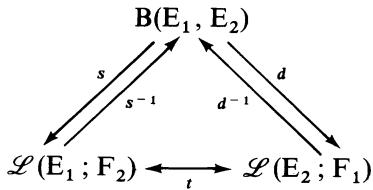
\includegraphics[keepaspectratio]{images/part001_08254dbd.jpg}}

其中 t 是转置同构（II, 第 46 页, 命题 5 及其推论）。鉴于 \(F_{1}\) 和 \(F_{2}\) 上弱拓扑的定义，立即可知：当给 \(\mathbf{B}(\mathbf{E}_{1}, \mathbf{E}_{2})\)、\(\mathcal{L}(\mathbf{E}_{1}; \mathbf{E}_{2})\) 和 \(\mathcal{L}(\mathbf{E}_{2}; \mathbf{F}_{1})\) 赋予简单收敛拓扑时，图 (3) 中的同构都是拓扑向量空间同构。

\subsection{Fréchet 空间乘积上的分别连续双线性映射}

命题 2. --- 设 E、F 和 G 是三个局部凸空间。假设 E 和 F 可度量化且 E 是桶型的。设 H 是从 E × F 到 G 中的分别连续双线性映射所成的一个集。假设对每个 x ∈ E，从 F 到 G 中的映射 u(x, .) 所成的集（u 取遍 H）是等度连续的。则 H 是等度连续的。

设 \(\mathrm{U}_n(\text{resp. } \mathrm{V}_n)\) 是 E（相应地，F）中 0 的邻域的一个基本序列。若 H 不等度连续，则存在 G 中 0 的一个闭的、凸的、均衡的邻域 W，使得对所有 \(n\)，\(\mathrm{H}(\mathrm{U}_n \times \mathrm{V}_n)\) 不含于 W。于是存在一个点对序列 \((x_n, y_n) \in \mathrm{U}_n \times \mathrm{V}_n\)，和 H 中元素的一个序列 \((u_n)\)，使得 \(u_n(x_n, y_n) \notin \mathrm{W}\)。设 \(p\) 是 W 的度规。对每个 \(y \in \mathrm{F}\) 和每个 \(u \in \mathrm{H}\)，从 E 到 G 中的映射 \(u(., y)\) 连续，因而 \(p \circ u(., y)\) 是 E 上的一个连续半范数。另一方面，对每个 \(x \in \mathrm{E}\)，映射 \(u(x, .)\)（对 \(u \in \mathrm{H}\)）所成的集是等度连续的；由于序列 \((y_n)\) 趋于 0，它是有界的，而所有 \(u(x, y_n)\)（对 \(n \geqslant 0\) 和 \(u \in \mathrm{H}\)）所成的集是有界的（III, 第 22 页, 命题 9）。由此可得，函数 \(p'(x) = \sup_{\substack{u \in \mathrm{H} \\ n \geqslant 0}} p(u(x, y_n))\) 是一个下半连续半

范数（有限的）于 E 上。由于 E 是桶型的，\(p'\) 连续（III, 第 24 页, 推论）。由于 \((x_{n})\) 在 E 中趋于 0，\(p'(x_{n})\) 趋于 0，故当 n 充分大时我们有 \(p'(x_{n}) \leqslant 1\)；但这时 \(p(u_{n}(x_{n}, y_{n})) \leqslant p'(x_{n}) \leqslant 1\)，因而 \(u_{n}(x_{n}, y_{n}) \in \mathbf{W}\)，这与关于 \(u_{n}, x_{n}, y_{n}\) 的假设矛盾。

推论 1. --- 设 E 和 F 是两个 Fréchet 空间，G 是一个局部凸空间。每个从 E × F 到 G 中的分别连续双线性映射都是连续的。

事实上，每个 Fréchet 空间都是桶型的（III, 第 25 页, 推论）。

设 E 和 F 是两个局部凸空间。我们用 \(\mathcal{B}(\mathrm{E},\mathrm{F})\) 记 \(E \times F\) 上的连续双线性型所成的空间，带上在形如 \(A \times B\) 的集上一致收敛的拓扑，其中 A（相应地，B）在 E（相应地，F）中有界。公式

\[
u (x, y) = \langle y, \phi (u) (x) \rangle
\]

（对 \(x \in \mathrm{E}\)、\(y \in \mathrm{F}\) 和 \(u \in \mathcal{B}(\mathrm{E}, \mathrm{F})\)）定义了一个连续线性单射 \(\phi\)，从 \(\mathcal{B}(\mathrm{E}, \mathrm{F})\) 到 \(\mathcal{L}_b(\mathrm{E}; \mathrm{F}_b')\) 中。

推论 2. --- 假设 E 和 F 可度量化且 E 是桶型的。则 \(\phi\) 是一个从 \(\mathcal{B}(\mathrm{E},\mathrm{F})\) 到 \(\mathcal{L}_b(\mathrm{E};\mathrm{F}_b')\) 上的拓扑向量空间同构。

设 \(f \in \mathcal{L}_b(\mathrm{E}; \mathrm{F}_b')\)。置 \(u(x, y) = \langle y, f(x) \rangle\)（对 \(x \in \mathrm{E}\) 和 \(y \in \mathrm{F}\)）。双线性型 \(u\)（在 \(\mathrm{E} \times \mathrm{F}\) 上的）是分别连续的；由命题 2，它属于 \(\mathcal{B}(\mathrm{E}, \mathrm{F})\)，且我们有 \(f = \phi(u)\)。因此 \(\phi\) 是一个从 \(\mathcal{B}(\mathrm{E}, \mathrm{F})\) 到 \(\mathcal{L}_b(\mathrm{E}; \mathrm{F}_b')\) 上的线性双射。立即可知 \(\phi\) 是双连续的，于是推论 2 得证。

\subsection{亚连续双线性映射}

在下面，我们将定义一个介于连续双线性映射的概念与分别连续双线性映射的概念之间的概念。

命题 3. --- 设 E、F、G 是三个局部凸空间，S 是 E 的有界子集的一个族。设 u 是从 E × F 到 G 中的一个分别连续双线性映射。下列性质等价：

\begin{enumerate}
\def\labelenumi{\alph{enumi})}
\item
  对 0 的每个邻域 \(\mathbf{W}\)（在 \(\mathbf{G}\) 中）和每个集 \(\mathbf{M} \in \mathfrak{S}\)，存在 0 的一个邻域 \(\mathbf{V}\)（在 \(\mathbf{F}\) 中），使得 \(u(\mathbf{M} \times \mathbf{V}) \subset \mathbf{W}\)。
\item
  对每个集 \(\mathbf{M} \in \mathfrak{S}\)，\(\mathbf{M}\) 在映射 \(x \mapsto u(x, .)\) 下的像是 \(\mathcal{L}(\mathrm{F}; \mathrm{G})\) 的一个等度连续子集。
\item
  映射 \(y \mapsto u(., y)\)（从 \(\mathbf{F}\) 到 \(\mathcal{L}_{\mathfrak{S}}(\mathbf{E}; \mathbf{G})\) 中）是连续的。
\item
  表明 \(y \mapsto u(., y)\) 在点 0 处连续，这是根据 \(\mathcal{L}_{\mathfrak{S}}(\mathrm{E}; \mathrm{G})\) 中 0 的邻域的定义（III, 第 13 页）；类似地，a) 表明 M 在映射 \(x \mapsto u(x, .)\) 下的像在点 0 处等度连续（III, 第 16 页）。
\end{enumerate}

定义 2. --- 设 u 是从 E × F 到 G 中的一个双线性映射。我们称 u 为 S-亚连续的，如果 u 分别连续且它满足命题 3 的等价条件 a)、b)、c) 之一。

命题 3 的条件 \(c)\) 表明，\(\mathfrak{S}\) -亚连续双线性映射的概念对 \(\mathfrak{S}\) 的依赖仅通过 \(\mathfrak{S}\) -拓扑（在 \(\mathcal{L}(\mathrm{E},\mathrm{G})\) 上的）实现。

对 F 的有界子集的每个集 T，我们类似地定义 T-亚连续映射的概念，只要在命题 3 中交换 E 与 F 的角色。称一个分别连续双线性映射 u 为 \((\mathfrak{S}, \mathfrak{T})\) -亚连续的，如果它既是 S-亚连续的又是 T-亚连续的。

每个从 \(E \times F\) 到 G 中的连续双线性映射对有界子集的集的每个对 \((\mathfrak{S}, \mathfrak{T})\) 都是 \((\mathfrak{S}, \mathfrak{T})\) -亚连续的：对 G 中 0 的每个邻域 W，存在 E 中 0 的一个邻域 U 和 F 中 0 的一个邻域 V，使得 \(u(U \times V) \subset W\)；由于每个集 \(M \in S\) 有界，存在 \(\lambda > 0\) 使得 \(\lambda M \subset V\)，于是

\[
u (\mathbf {M} \times \lambda \mathbf {V}) = u (\lambda \mathbf {M} \times \mathbf {V}) \subset u (\mathbf {U} \times \mathbf {V}) \subset \mathbf {W}.
\]

逆命题一般不成立（III, 第 47 页, 习题 3）。

命题 4. --- 设 u 是从 E × F 到 G 中的一个 S-亚连续双线性映射。对每个集 M ∈ S，u 在 M × F 上的限制是连续的，且对 F 的每个有界子集 Q，u(M × Q) 在 G 中有界。

第一个断言由 GT, X, § 2, No.~1 的推论 3 得出。设 W 是 G 中 0 的一个邻域；由假设，存在 F 中 0 的一个邻域 V，使得 \(u(\mathbf{M} \times \mathbf{V}) \subset \mathbf{W}\)。由于存在 \(\lambda \neq 0\) 使得 \(\lambda \mathbf{Q} \subset \mathbf{V}\)，我们有 \(\lambda u(\mathbf{M} \times \mathbf{Q}) = u(\mathbf{M} \times \lambda \mathbf{Q}) \subset \mathbf{W}\)，这就证明了命题的第二部分。

命题 5. --- 设 u 是从 E × F 到 G 中的一个 (S, T)-亚连续双线性映射。对每对集 M ∈ S、N ∈ T，u 在 M × N 上一致连续。命题由 GT, X, § 2, No.~1 的命题 2 和 GT, X, § 2, No.~2 的命题 5 立即得出。

命题 6. --- 若 F 是桶型空间，则每个从 E × F 到局部凸空间 G 中的分别连续双线性映射 u 对 E 的有界子集的每个集 S 都是 S-亚连续的。

换言之，线性映射 \(y \mapsto u(., y)\)（从 \(F\) 到 \(\mathcal{L}_b(E; G)\) 中）是连续的。只需（III, 第 30 页, 命题 3）证明：每个有界子集 \(M\)（\(E\) 的）在 \(x \mapsto u(x, .)\) 下的像在 \(\mathcal{L}(F; G)\) 中等度连续。但由命题 1（III, 第 28 页），这个像是 \(\mathcal{L}(F; G)\) 的一个简单有界子集，而由于 \(F\) 是桶型的，\(\mathcal{L}(F; G)\) 的每个简单有界子集都是等度连续的（III, 第 25 页, 定理 1）。

评注. --- 假设 F 的拓扑是 F 上使线性映射 \(h_{\alpha}:F_{\alpha}\to F\) 连续的最细局部凸拓扑（II, 第 27 页）。则命题 3 的条件 c)（III, 第 30 页）表明：若 E 和 G 是局部凸的，则双线性映射 \(u:E\times F\to G\) 是 S-亚连续的，当且仅当诸双线性映射

\[
(x, y _ {\alpha}) \mapsto u (x, h _ {\alpha} (y _ {\alpha}))
\]

（从 \(\mathbf{E} \times \mathbf{F}_{\alpha}\) 到 \(\mathbf{G}\) 中）中的每一个都是 \(\mathfrak{S}\) -亚连续的。

现在假设 \(\mathbf{E}\) 是一个局部凸空间，它是闭向量子空间的一个递增序列 \((\mathbf{E}_n)\)（\(\mathbf{E}\) 的）的严格归纳极限（II, 第 33 页）；则每个集 \(\mathbf{M} \in \mathfrak{S}\) 含于诸 \(\mathbf{E}_n\) 之一且在这个子空间中有界（III, 第 5 页, 命题 6）。我们用 \(\mathfrak{S}_n\) 记属于 \(\mathfrak{S}\) 且含于 \(\mathbf{E}_n\) 的所有子集所成的族。

命题 3 的条件 a)（III, 第 30 页）表明：为使双线性映射 \(u: \mathrm{E} \times \mathrm{F} \to \mathrm{G}\) 是 \(\mathfrak{S}\) -亚连续的，必要且充分的是诸限制 \(u_n: \mathrm{E}_n \times \mathrm{F} \to \mathrm{G}\)（\(u\) 的）中的每一个都是 \(\mathfrak{S}_n\) -亚连续的。

\subsection{亚连续双线性映射的扩张}

命题 7. --- 设 E、F、G 是三个局部凸空间，其中 G 假设为 Hausdorff 的；设 \(E_{0}\)（相应地，\(F_{0}\)）是 E（相应地，F）的一个稠密向量子空间。设 u 是从 \(E \times F\) 到 G 中的一个分别连续双线性映射。

\begin{enumerate}
\def\labelenumi{\arabic{enumi})}
\item
  若 \(u(\mathrm{E}_0 \times \mathrm{F}_0) = \{0\}\)，则 \(u = 0\)。
\item
  设 \(\mathfrak{S}_0\) 是 \(\mathbf{E}_0\) 的有界子集的一个族；若 \(u\) 在 \(\mathbf{E}_0 \times \mathbf{F}_0\) 上的限制是 \(\mathfrak{S}_0\) -亚连续的，则 \(u\) 本身也是。
\item
  由假设，对所有 \(x \in \mathrm{E}_0\)，连续线性映射 \(u(x, .)\) 在 \(\mathrm{F}_0\) 上为零，从而在 \(\mathrm{F}\) 上为零：因此对所有 \(y \in \mathrm{F}\)，连续线性映射 \(u(., y)\) 在 \(\mathrm{E}_0\) 上为零，从而在 \(\mathrm{E}\) 上为零。这就证明 \(u = 0\)。
\item
  对 G 中 0 的每个闭邻域 W 和每个集 \(\mathbf{M} \in \mathfrak{S}_0\)，由假设，存在 \(\mathrm{F}_0\) 中 0 的一个邻域 V，使得 \(u(\mathbf{M} \times \mathbf{V}) \subset \mathbf{W}\)。但 \(\overline{\mathbf{V}}\) 是 F 中 0 的一个邻域；对每个 \(x \in \mathbf{M}\)，关系 \(u(\{x\} \times \mathbf{V}) \subset \mathbf{W}\) 蕴含 \(u(\{x\} \times \overline{\mathbf{V}}) \subset \mathbf{W}\)，因为 \(u(x, .)\) 连续且 W 是闭的；因此 \(u(\mathbf{M} \times \overline{\mathbf{V}}) \subset \mathbf{W}\)，这就证明 \(u\) 是 \(\mathfrak{S}_0\) -亚连续的。
\end{enumerate}

命题 8. --- 设 E、F、G 是三个局部凸空间；假设 G 是 Hausdorff 且拟完备的。设 \(E_{0}\)（相应地，\(F_{0}\)）是 E（相应地，F）的一个稠密向量子空间，\(S_{0}\)（相应地，\(T_{0}\)）是 \(E_{0}\)（相应地，\(F_{0}\)）的有界子集的一个族，使得 E（相应地，F）的每个点都在 \(S_{0}\)（相应地，\(T_{0}\)）的某个元素的闭包中。则每个 \((\mathfrak{S}_{0}, \mathfrak{T}_{0})\) -亚连续双线性映射 u（从 \(E_{0} \times F_{0}\) 到 G 中的）都唯一地扩张为从 E × F 到 G 中的一个分别连续双线性映射 \(\overline{u}\)，且 \(\overline{u}\) 是 \((\mathfrak{S}_{0}, \mathfrak{T}_{0})\) -亚连续的。

\(\overline{u}\) 的唯一性和亚连续性由命题 7 得出；剩下要证明 \(\overline{u}\) 的存在性。对每个 \(y' \in F_{0}\)，连续线性映射 \(x' \mapsto u(x', y')\)（从 \(E_{0}\) 到 G 中的）唯一地扩张为一个连续线性映射 \(x \mapsto u_{1}(x, y')\)（从 E 到 G 中的）（III, 第 8 页, 命题 10）。立即由此可得，对每个 \(x \in E\)，映射 \(y' \mapsto u_{1}(x, y')\)（从 \(F_{0}\) 到 G 中的）是线性的；我们将证明它是连续的。由假设，存在 \(M \in S_{0}\)，使得 \(x \in M\)。对 G 中 0 的每个闭邻域 W，由假设，存在 \(F_{0}\) 中 0 的一个邻域 V，使得 \(u(M \times V) \subset W\)；由于 \(x \mapsto u_{1}(x, y')\) 连续，我们推出 \(u_{1}(\overline{\mathbf{M}} \times \mathbf{V}) \subset \mathbf{W}\)，特别地，\(u_{1}(x, y') \in \mathbf{W}\)（对所有 \(y' \in V\)）。这就确立了我们的断言。由命题 7，双线性映射 \(u_{1}\)（从 \(E \times F_{0}\) 到 G 中的）是 \((\mathfrak{S}_{0}, \mathfrak{T}_{0})\) -亚连续的。我们把证明结束于：在证明的第一部分中交换 E 与 F 的角色并应用于 \(u_{1}\)。
